% =====================================================================
% Academic Internship Report — Rainfull Cartagen
% =====================================================================
\documentclass[12pt,a4paper]{report}

% ---- Essential Packages ----
\usepackage[utf8]{inputenc}
\usepackage[T1]{fontenc}
\usepackage[english]{babel}
\usepackage{geometry}
\geometry{left=2.5cm, right=2.5cm, top=2.5cm, bottom=2.5cm}
\usepackage{graphicx}
\usepackage{float}
\usepackage{caption}
\usepackage{subcaption}
\usepackage{amsmath,amssymb}
\usepackage{hyperref}
\hypersetup{
    colorlinks=true,
    linkcolor=blue!70!black,
    citecolor=blue!70!black,
    urlcolor=blue!80!black
}
\usepackage{setspace}
\onehalfspacing
\usepackage{titlesec}
\usepackage{tocloft}
\usepackage{fancyhdr}
\usepackage{array}
\usepackage{booktabs}
\usepackage{longtable}
\usepackage{enumitem}
\usepackage{xcolor}
\usepackage{listings}
\usepackage{tikz}
\usetikzlibrary{shapes.geometric, arrows.meta, positioning, fit, calc}

% ---- Code listings style ----
\lstdefinestyle{pythonstyle}{
  language=Python,
  basicstyle=\ttfamily\footnotesize,
  keywordstyle=\color{blue!70!black}\bfseries,
  stringstyle=\color{red!60!black},
  commentstyle=\color{green!50!black}\itshape,
  numbers=left,
  numberstyle=\tiny\color{gray},
  frame=single,
  breaklines=true,
  captionpos=b,
  tabsize=4
}
\lstdefinestyle{sqlstyle}{
  language=SQL,
  basicstyle=\ttfamily\footnotesize,
  keywordstyle=\color{blue!70!black}\bfseries,
  stringstyle=\color{red!60!black},
  commentstyle=\color{green!50!black}\itshape,
  numbers=left,
  numberstyle=\tiny\color{gray},
  frame=single,
  breaklines=true,
  captionpos=b,
  tabsize=4
}

% ---- Header/Footer ----
\pagestyle{fancy}
\fancyhf{}
\fancyhead[L]{\small\leftmark}
\fancyhead[R]{\small Rainfull Cartagen --- DGRE}
\fancyfoot[C]{\thepage}
\renewcommand{\headrulewidth}{0.4pt}
\renewcommand{\footrulewidth}{0.2pt}

% ---- Chapter title style ----
\titleformat{\chapter}[display]
  {\normalfont\Large\bfseries\centering}
  {\chaptertitlename\ \thechapter}{15pt}{\LARGE}

\begin{document}

% =====================================================================
% COVER PAGE
% =====================================================================
\begin{titlepage}
\begin{center}

\textbf{\large Republic of Tunisia}\\[0.15cm]
\textbf{\large Ministry of Higher Education and Scientific Research}\\[0.15cm]
\textbf{\large University of Tunis El Manar}\\[0.15cm]
\textbf{\Large École Nationale d'Ingénieurs de Tunis (ENIT)}\\[0.4cm]

\rule{\linewidth}{0.6pt}\\[0.4cm]

{\Large\textbf{ENGINEERING INTERNSHIP REPORT}}\\[0.25cm]
{\large Submitted in Partial Fulfilment of the Requirements for the}\\[0.15cm]
{\large National Engineering Diploma}\\[0.5cm]

\rule{\linewidth}{0.4pt}\\[0.6cm]

{\Huge\textbf{Rainfull Cartagen:}}\\[0.4cm]
{\LARGE\textbf{Intelligent Multi-Agent Platform for Automated Pluviometric Yearbook Generation and Hydrological Knowledge Management}}\\[0.6cm]

\rule{\linewidth}{0.4pt}\\[0.8cm]

\begin{minipage}{0.85\textwidth}
\begin{tabular}{ll}
\textbf{Author:} & \textbf{Dhia Eddine BARHOUMI} \\[0.3cm]
\textbf{Institutional Supervisor:} & \textbf{Alaa Eddine JELASSI} \\[0.3cm]
\textbf{Host Organization:} & \textbf{Direction Générale des Ressources en Eau (DGRE)} \\[0.3cm]
\textbf{Host Department:} & Sous-Direction de l'Hydrologie Analytique \\[0.3cm]
\textbf{Academic Year:} & 2024 / 2025 \\[0.3cm]
\textbf{Internship Period:} & June 15 -- July 30, 2026 \\
\end{tabular}
\end{minipage}

\vfill

\textbf{Ministry of Agriculture, Water Resources and Fisheries (MARHP)}\\
General Directorate of Water Resources (DGRE)\\
43, Rue de la Manoubia, Montfleury, 1008 Tunis, Tunisia

\end{center}
\end{titlepage}

% =====================================================================
% DEDICATION
% =====================================================================
\chapter*{Dedication}
\addcontentsline{toc}{chapter}{Dedication}
\thispagestyle{empty}

\vspace{3cm}
\begin{center}
\textit{
To my beloved parents, whose endless sacrifices, continuous prayers, and unwavering support have illuminated every step of my academic journey.\\[0.6cm]
To my professors and instructors at the École Nationale d'Ingénieurs de Tunis (ENIT), who imparted the knowledge, technical discipline, and problem-solving passion that formed my engineering mindset.\\[0.6cm]
To my supervisor, Mr. Alaa Eddine JELASSI, and the dedicated hydrologists and technicians at the General Directorate of Water Resources (DGRE), whose commitment to monitoring and protecting Tunisia's vital water resources inspires rigorous and impactful engineering.\\[0.6cm]
To all my friends and colleagues who stood by me throughout this challenging and rewarding experience.
}
\end{center}
\newpage

% =====================================================================
% ACKNOWLEDGEMENTS
% =====================================================================
\chapter*{Acknowledgements}
\addcontentsline{toc}{chapter}{Acknowledgements}

I would like to express my deepest and most sincere gratitude to my supervisor at the General Directorate of Water Resources (DGRE), \textbf{Mr. Alaa Eddine JELASSI}, for his continuous availability, exemplary guidance, and constant constructive feedback throughout the entire internship. His in-depth mastery of hydrological data workflows and strategic vision for institutional modernization provided an invaluable compass for the design and execution of the \textbf{Rainfull Cartagen} platform.

I extend my profound appreciation to the management and engineering teams of the \textbf{Direction Générale des Ressources en Eau (DGRE)}, particularly the \textit{Sous-Direction de l'Hydrologie Analytique} and the \textit{Direction des Eaux de Surface}, for their welcoming reception, their willingness to share decades of institutional knowledge, and their valuable technical insights regarding the historical compilation of the national pluviometric yearbook.

I also express my gratitude to the administrative and academic staff of the \textbf{École Nationale d'Ingénieurs de Tunis (ENIT)}, University of Tunis El Manar, for the solid theoretical foundations, research rigor, and engineering methodology that enabled me to tackle complex geospatial, algorithmic, and artificial intelligence challenges.

Finally, I acknowledge the global open-source community behind the fundamental technologies powering this project --- including PostgreSQL/PostGIS, Python, FastAPI, GeoPandas, Matplotlib, SciPy, and the open-weights Large Language Model ecosystems --- whose collaborative efforts democratize cutting-edge computing tools for public resource governance.

\newpage

% =====================================================================
% ABSTRACT
% =====================================================================
\chapter*{Abstract}
\addcontentsline{toc}{chapter}{Abstract}

In semi-arid Mediterranean regions like Tunisia, water resources are under acute climatic and anthropogenic stress, with agriculture consuming approximately 80\% of available water reserves. The General Directorate of Water Resources (DGRE), operating under the Ministry of Agriculture, Water Resources and Fisheries (MARHP), is legally mandated to observe, analyze, and publish national hydrological records. Its flagship publication, the \textit{Annuaire Pluviométrique de la Tunisie}, consolidates daily rainfall observations across 148 national reference stations distributed throughout 24 governorates and 6 natural regions. Historically, this publication pipeline was entirely manual, relying on fragmented Microsoft Access (.mdb) files, spreadsheet calculations, and semi-manual desktop GIS drafting, requiring \textbf{7 to 8 months} of intensive human labor and presenting substantial vulnerability to formatting and calculation discrepancies.

This internship project presents the conception, architecture, implementation, and deployment of \textbf{Rainfull Cartagen}, an intelligent multi-agent platform that fully automates the national pluviometric yearbook pipeline while delivering natural language querying capabilities backed by Retrieval-Augmented Generation (RAG) and Fine-Tuning. The system transitions the DGRE data architecture from disparate desktop databases to a spatialized \textbf{PostgreSQL/PostGIS} repository. It formalizes official hydrological calculations into automated, high-precision Python engines implementing the \textbf{Thiessen Polygon method} (Voronoi surface integration) for regional and national weighted averages, and \textbf{Inverse Distance Weighting (IDW)} on a $300 \times 300$ grid for continuous isohyet cartography.

To empower non-programmer hydrologists, Rainfull Cartagen introduces a \textbf{deliberative multi-agent architecture} operating under a Supervisor Pattern. The platform orchestrates specialized agents: a \textit{CartaGenOrchestrator} for intent dispatching, a \textit{SQLGeneratorAgent} translating natural language into spatialized SQL, a \textit{SIGGeneratorAgent} synthesizing geospatial visualization scripts from parameterized templates, a \textit{QualityVerificationAgent} driving a closed self-correction loop via Abstract Syntax Tree (AST) static inspection and isolated sandbox execution, and an \textit{AnnuaireRAGAgent} backed by an in-process vector database (\textit{Zvec}) with temporal filtering and a +30\% spatial proximity boost. 

Rainfull Cartagen compresses the entire production timeline of the official 100+ page publication-grade PDF yearbook from \textbf{7--8 months to under 3 minutes}, achieving 100\% mathematical parity with official DGRE historical reference publications. The platform is containerized using Docker Compose for reliable on-premises intranet deployment.

\vspace{0.6cm}
\noindent\textbf{Keywords:} Rainfull Cartagen, DGRE Tunisia, Pluviometric Yearbook, Multi-Agent Systems, Knowledge Management (KMS), PostgreSQL/PostGIS, Thiessen Polygons, IDW Interpolation, Retrieval-Augmented Generation (RAG), LoRA Fine-Tuning, AST Security Sandbox, LaTeX Automation.

\newpage

% =====================================================================
% TABLES OF CONTENTS, FIGURES, TABLES, ABBREVIATIONS
% =====================================================================
\tableofcontents
\newpage
\listoffigures
\newpage
\listoftables
\newpage

\chapter*{List of Abbreviations}
\addcontentsline{toc}{chapter}{List of Abbreviations}

\begin{longtable}{ll}
\textbf{AI} & Artificial Intelligence \\
\textbf{API} & Application Programming Interface \\
\textbf{AST} & Abstract Syntax Tree \\
\textbf{BI} & Business Intelligence \\
\textbf{CLI} & Command Line Interface \\
\textbf{CRDA} & Commissariat Régional de Développement Agricole \\
\textbf{CRS} & Coordinate Reference System \\
\textbf{CRUD} & Create, Read, Update, Delete \\
\textbf{CSS} & Cascading Style Sheets \\
\textbf{DGRE} & Direction Générale des Ressources en Eau \\
\textbf{DPI} & Dots Per Inch \\
\textbf{EPSG} & European Petroleum Survey Group (Geodetic Parameter Registry) \\
\textbf{ER} & Entity-Relationship \\
\textbf{ETL} & Extract, Transform, Load \\
\textbf{FAO} & Food and Agriculture Organization of the United Nations \\
\textbf{GIS} & Geographic Information System \\
\textbf{GiST} & Generalized Search Tree (PostgreSQL Index) \\
\textbf{HNSW} & Hierarchical Navigable Small World (Vector Index) \\
\textbf{HTML} & HyperText Markup Language \\
\textbf{HTTP} & HyperText Transfer Protocol \\
\textbf{IDW} & Inverse Distance Weighting \\
\textbf{JSON} & JavaScript Object Notation \\
\textbf{KM} & Knowledge Management \\
\textbf{KMC} & Knowledge Management Cycle \\
\textbf{KMS} & Knowledge Management System \\
\textbf{LLM} & Large Language Model \\
\textbf{LoRA} & Low-Rank Adaptation \\
\textbf{MARHP} & Ministère de l'Agriculture, des Ressources Hydrauliques et de la Pêche \\
\textbf{MCD} & Modèle Conceptuel de Données (Conceptual Data Model) \\
\textbf{MERISE} & Méthode d'Étude et de Réalisation Informatique pour les Systèmes d'Entreprise \\
\textbf{ONAGRI} & Observatoire National de l'Agriculture \\
\textbf{OWASP} & Open Worldwide Application Security Project \\
\textbf{PDF} & Portable Document Format \\
\textbf{PEFT} & Parameter-Efficient Fine-Tuning \\
\textbf{PESTEL} & Political, Economic, Sociocultural, Technological, Environmental, Legal \\
\textbf{PostGIS} & PostgreSQL Geographic Information System Extension \\
\textbf{RAG} & Retrieval-Augmented Generation \\
\textbf{REST} & Representational State Transfer \\
\textbf{SECI} & Socialization, Externalization, Combination, Internalization \\
\textbf{SGBD} & Système de Gestion de Base de Données (DBMS) \\
\textbf{SIG} & Système d'Information Géographique (GIS) \\
\textbf{SQL} & Structured Query Language \\
\textbf{SWOT} & Strengths, Weaknesses, Opportunities, Threats \\
\textbf{UI} & User Interface \\
\textbf{UML} & Unified Modeling Language \\
\textbf{UTM} & Universal Transverse Mercator (UTM Zone 32N) \\
\textbf{UX} & User Experience \\
\end{longtable}

\newpage

% =====================================================================
% GENERAL INTRODUCTION
% =====================================================================
\chapter*{General Introduction}
\addcontentsline{toc}{chapter}{General Introduction}

\section*{I. Contextual Background: Water Scarcity and National Governance}

Water security is universally recognized as the foundational pillar of socio-economic stability, agricultural autonomy, and environmental resilience in the Mediterranean basin. In Tunisia, a country characterized by predominantly arid and semi-arid bioclimatic zones, water management constitutes a critical strategic imperative \cite{fao2022, elgourari2024}. The agricultural sector alone accounts for nearly 80\% of national water consumption \cite{onagri2023}, placing extreme reliance on interannual rainfall patterns that exhibit dramatic spatial disparities and high temporal variability.

Under the institutional framework established by the Tunisian state \cite{jort2001}, the \textbf{Direction Générale des Ressources en Eau (DGRE)}, operating under the Ministry of Agriculture, Water Resources and Fisheries (MARHP), serves as the sovereign national authority responsible for observing, assessing, archiving, and disseminating hydrological data \cite{dgre2023}. Among its fundamental duties, the DGRE annually publishes the official \textit{Annuaire Pluviométrique de la Tunisie} (National Rainfall Yearbook). This institutional document compiles, cleanses, validates, and synthesizes precipitation records from a certified network of \textbf{148 reference stations} distributed across the \textbf{24 governorates} and \textbf{6 natural regions} of the Republic.

\section*{II. Problem Statement: The Manual Bottleneck and Data Fragmentation}

Despite the critical strategic value of rainfall data for irrigation scheduling, dam operations, drought response policies, and hydraulic engineering projects, the historical workflow employed by the DGRE to produce the annual yearbook suffers from severe structural limitations:

\begin{enumerate}[label=\textbf{\arabic*.}]
  \item \textbf{Prohibitive Production Latency}: The collection, cross-verification, statistical consolidation, and cartographic drafting of the annual yearbook required \textbf{7 to 8 months} of intensive, manual effort by specialized technicians and engineers. Consequently, national rainfall reports were frequently published nearly a year after the conclusion of the hydrological cycle.
  \item \textbf{Severe Data Fragmentation}: Rainfall records originated from 24 regional agricultural commissariats (CRDAs), compiled in decentralized and heterogeneous Microsoft Access (.mdb) files and manual spreadsheets with no unified schema, transactional consistency, or automated synchronization.
  \item \textbf{Total Absence of Spatial Database Capabilities}: Legacy desktop DBMS tools (such as MS Access) cannot natively represent spatial geometries, perform geodetic coordinate transformations, or execute spatial overlay queries, forcing technicians to export data into external GIS packages (e.g., Surfer, ArcView, QGIS) through cumbersome manual steps.
  \item \textbf{Human Error and Calculation Vulnerabilities}: Calculating official surface-weighted precipitation averages (using the Thiessen polygon method) and plotting isohyet contours relied on semi-automated spreadsheet formulas and manually traced contours, introducing human error risks and inconsistencies across successive yearbooks.
  \item \textbf{Absence of Natural Language Accessibility}: Decision-makers, agronomists, and researchers possessed no interactive interface to query the hydrological repository directly in natural language; extracting specific historical statistics required manual database querying by IT staff.
\end{enumerate}

\section*{III. Objectives and Scope of the Project}

To address these challenges comprehensively, this engineering internship project focuses on the conceptualization, development, and on-premises deployment of \textbf{Rainfull Cartagen}, an end-to-end intelligent platform engineered to transform the DGRE's rainfall information pipeline. The project encompasses four primary engineering objectives:

\begin{itemize}
  \item \textbf{Unified Spatial Data Infrastructure}: Migrate fragmented Access databases into a normalized, enterprise-grade \textbf{PostgreSQL/PostGIS} repository, preserving 148 reference stations, historical daily observations, 50-year interannual normals (1959--2009), and official administrative boundaries in the projected UTM Zone 32N (EPSG:32632) coordinate system.
  \item \textbf{Rigorous Hydrological Algorithm Engine}: Implement and validate official DGRE statistical formulas as reproducible Python modules, including the \textbf{Thiessen polygon method} (Voronoi surface weighting) for regional water balance tables and \textbf{vectorized Inverse Distance Weighting (IDW)} for continuous isohyet mapping.
  \item \textbf{Deliberative Multi-Agent AI System}: Design an autonomous multi-agent pipeline adhering to the Supervisor Pattern, incorporating specialized agents for intent routing, Text-to-SQL generation, Python GIS script synthesis, vector-based Retrieval-Augmented Generation (RAG), and a closed self-correction loop powered by Abstract Syntax Tree (AST) security validation.
  \item \textbf{Automated Publication-Ready LaTeX Generation}: Engineer a modular document assembly engine capable of compiling a complete, 100+ page official PDF yearbook matching DGRE visual standards in \textbf{under 3 minutes}.
\end{itemize}

\section*{IV. Structure of the Report}

The remainder of this report is organized into four detailed chapters:
\begin{itemize}
  \item \textbf{Chapter I --- The DGRE and the Hydrological Context of Tunisia}: Establishes the institutional mandate of the DGRE, examines the national rainfall monitoring network across the 6 natural regions, details the contents of the official yearbook, and conducts a diagnosis of the legacy manual workflow.
  \item \textbf{Chapter II --- Literature Review and Theoretical Foundations}: Reviews knowledge management theory (Tuomi's hierarchy, Nonaka's SECI model, KM cycles, organizational memory), the Design Thinking methodology, spatial statistics (Thiessen vs. IDW), multi-agent LLM systems, RAG, LoRA fine-tuning, and defensive sandboxing.
  \item \textbf{Chapter III --- System Analysis, Modeling, and Architecture}: Details stakeholder requirements, MERISE conceptual modeling, the database migration strategy, the Clean/Hexagonal multi-agent architecture, algorithmic formulations, and the AST defensive security model.
  \item \textbf{Chapter IV --- Implementation, Experimental Results, and Deployment}: Chronologically chronicles the development milestones (from the internship journal), details AI fine-tuning and data rebalancing, showcases cartographic and tabular outputs, presents validation against official DGRE archives, and details Docker containerization.
\end{itemize}

\newpage

% =====================================================================
% CHAPTER I: DGRE AND HYDROLOGICAL CONTEXT
% =====================================================================
\chapter{The DGRE and the Hydrological Context of Tunisia}

\section{Introduction}

This chapter details the institutional framework, missions, and operational organization of the General Directorate of Water Resources (DGRE). It then analyzes the spatial characteristics of Tunisia's rainfall observation network, introduces the structure of the official \textit{Annuaire Pluviométrique}, and formally diagnoses the limitations of the legacy manual workflow.

\section{Missions and Organizational Structure of the DGRE}

\subsection{Institutional Mandate}
The General Directorate of Water Resources (DGRE) is the executive technical authority under the Ministry of Agriculture, Water Resources and Fisheries (MARHP), established by national decree \cite{jort2001} to govern the quantitative and qualitative evaluation of surface and groundwater across the Tunisian territory. Its foundational responsibilities include \cite{dgre2023}:
\begin{itemize}
  \item Planning and operating the national hydrometric and pluviometric observation networks.
  \item Centralizing, archiving, validating, and publishing official national hydrological statistics.
  \item Formulating water balances to support national planning for hydraulic infrastructure (dams, transfers, artificial groundwater recharge).
  \item Providing technical expertise during extreme hydrological events (floods and prolonged meteorological droughts).
\end{itemize}

\subsection{Organizational Hierarchy}
To execute its mandate, the DGRE is structured into specialized technical directorates and sub-directorates:
\begin{itemize}
  \item \textbf{Direction des Eaux de Surface (Surface Water Directorate)}: Oversees analytical hydrology, river hydrometry, flood risk management, and the publication of annual statistical yearbooks.
  \item \textbf{Sous-Direction de l'Hydrologie Analytique}: The specific host unit for this internship, responsible for processing raw rainfall measurements, verifying data coherence, executing spatial interpolations, and formatting the annual pluviometric yearbook.
  \item \textbf{Direction des Eaux Souterraines (Groundwater Directorate)}: Manages piezometric observation networks, deep aquifers, and artificial water table recharge monitoring.
  \item \textbf{Sous-Direction des Réseaux et de la Maintenance}: Ensures physical upkeep and sensor calibration across the 24 regional commissariats (CRDAs).
\end{itemize}

At the regional tier, the 24 \textbf{Commissariats Régionaux de Développement Agricole (CRDAs)} operate field observation stations, collecting daily rain gauge records and transmitting monthly digests to the central DGRE headquarters in Tunis.

\section{The National Rainfall Monitoring Network}

\subsection{The 148 Reference Stations}
Although hundreds of rainfall gauges exist nationwide, the DGRE relies on a core, certified network of \textbf{148 national reference stations} for official reporting. These 148 stations possess long-term historical records (dating back to the 1950s) necessary for computing rigorous 50-year climatological normals (1959--2009). The geographical coordinates of these stations are officially registered in the Universal Transverse Mercator (UTM) Zone 32 North projection based on the WGS84 ellipsoid (EPSG:32632).

Figure~\ref{fig:reseau_stations} illustrates the national spatial distribution of the 148 reference stations. As demonstrated by the map, the observation network exhibits marked spatial heterogeneity: the northern governorates contain a dense network of stations due to mountainous topography and high rainfall frequency, while the southern Saharan governorates exhibit a sparse network reflecting vast desert expanses.

\begin{figure}[htbp]
    \centering
    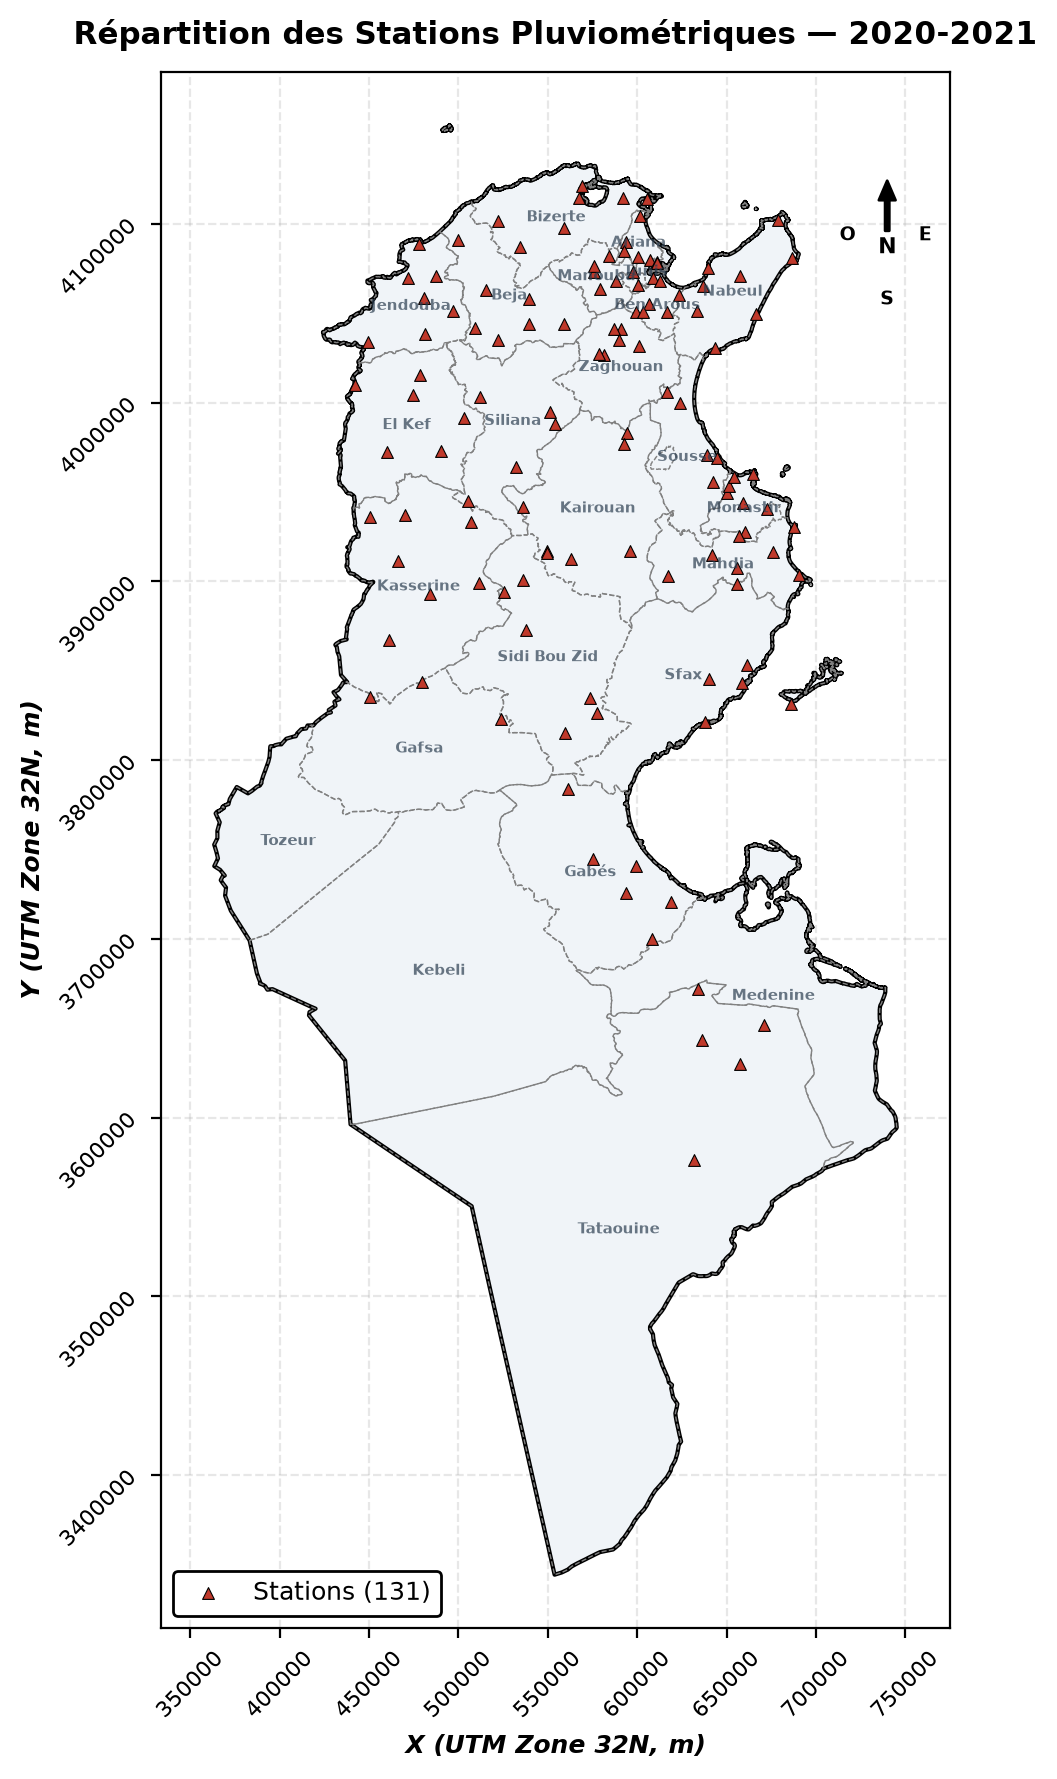
\includegraphics[width=0.72\textwidth]{figures/carte_reseau_148_stations.png}
    \caption{Spatial distribution of the 148 national reference pluviometric stations of the DGRE (Projected in UTM Zone 32N / EPSG:32632).}
    \label{fig:reseau_stations}
\end{figure}

\subsection{The Six Natural Regions of Tunisia}
Hydrologists at the DGRE divide the Tunisian territory into \textbf{six homogeneous Natural Regions} for water balance computation and climatological synthesis \cite{elgourari2024}. This division accounts for the Atlas mountain ridge (Dorsale Tunisienne), marine influences, and Saharan desert boundaries:
\begin{enumerate}
  \item \textbf{Nord Ouest (North West)}: High-rainfall mountainous region (Kroumirie, Medjerda valley) comprising Jendouba, Béja, Le Kef, and Siliana ($16,517\text{ km}^2$).
  \item \textbf{Nord Est (North East)}: Coastal agricultural plains including Tunis, Ariana, Ben Arous, Manouba, Nabeul, Zaghouan, and Bizerte ($11,725\text{ km}^2$).
  \item \textbf{Centre Ouest (Central West)}: Semi-arid steppes encompassing Kairouan, Kasserine, and Sidi Bouzid ($22,184\text{ km}^2$).
  \item \textbf{Centre Est (Central East)}: Coastal Sahelian plain including Sousse, Monastir, Mahdia, and Sfax ($13,430\text{ km}^2$).
  \item \textbf{Sud Ouest (South West)}: Arid oasis and Chott depression region including Gafsa, Tozeur, and Kébili ($35,761\text{ km}^2$).
  \item \textbf{Sud Est (South East)}: Pre-Saharan desert and Jeffara plain comprising Gabès, Médenine, and Tataouine ($55,305\text{ km}^2$).
\end{enumerate}

Figure~\ref{fig:regions_naturelles} displays the geographical boundaries of these 6 Natural Regions. Table~\ref{tab:regions} details their territorial extent and administrative governorates.

\begin{figure}[htbp]
    \centering
    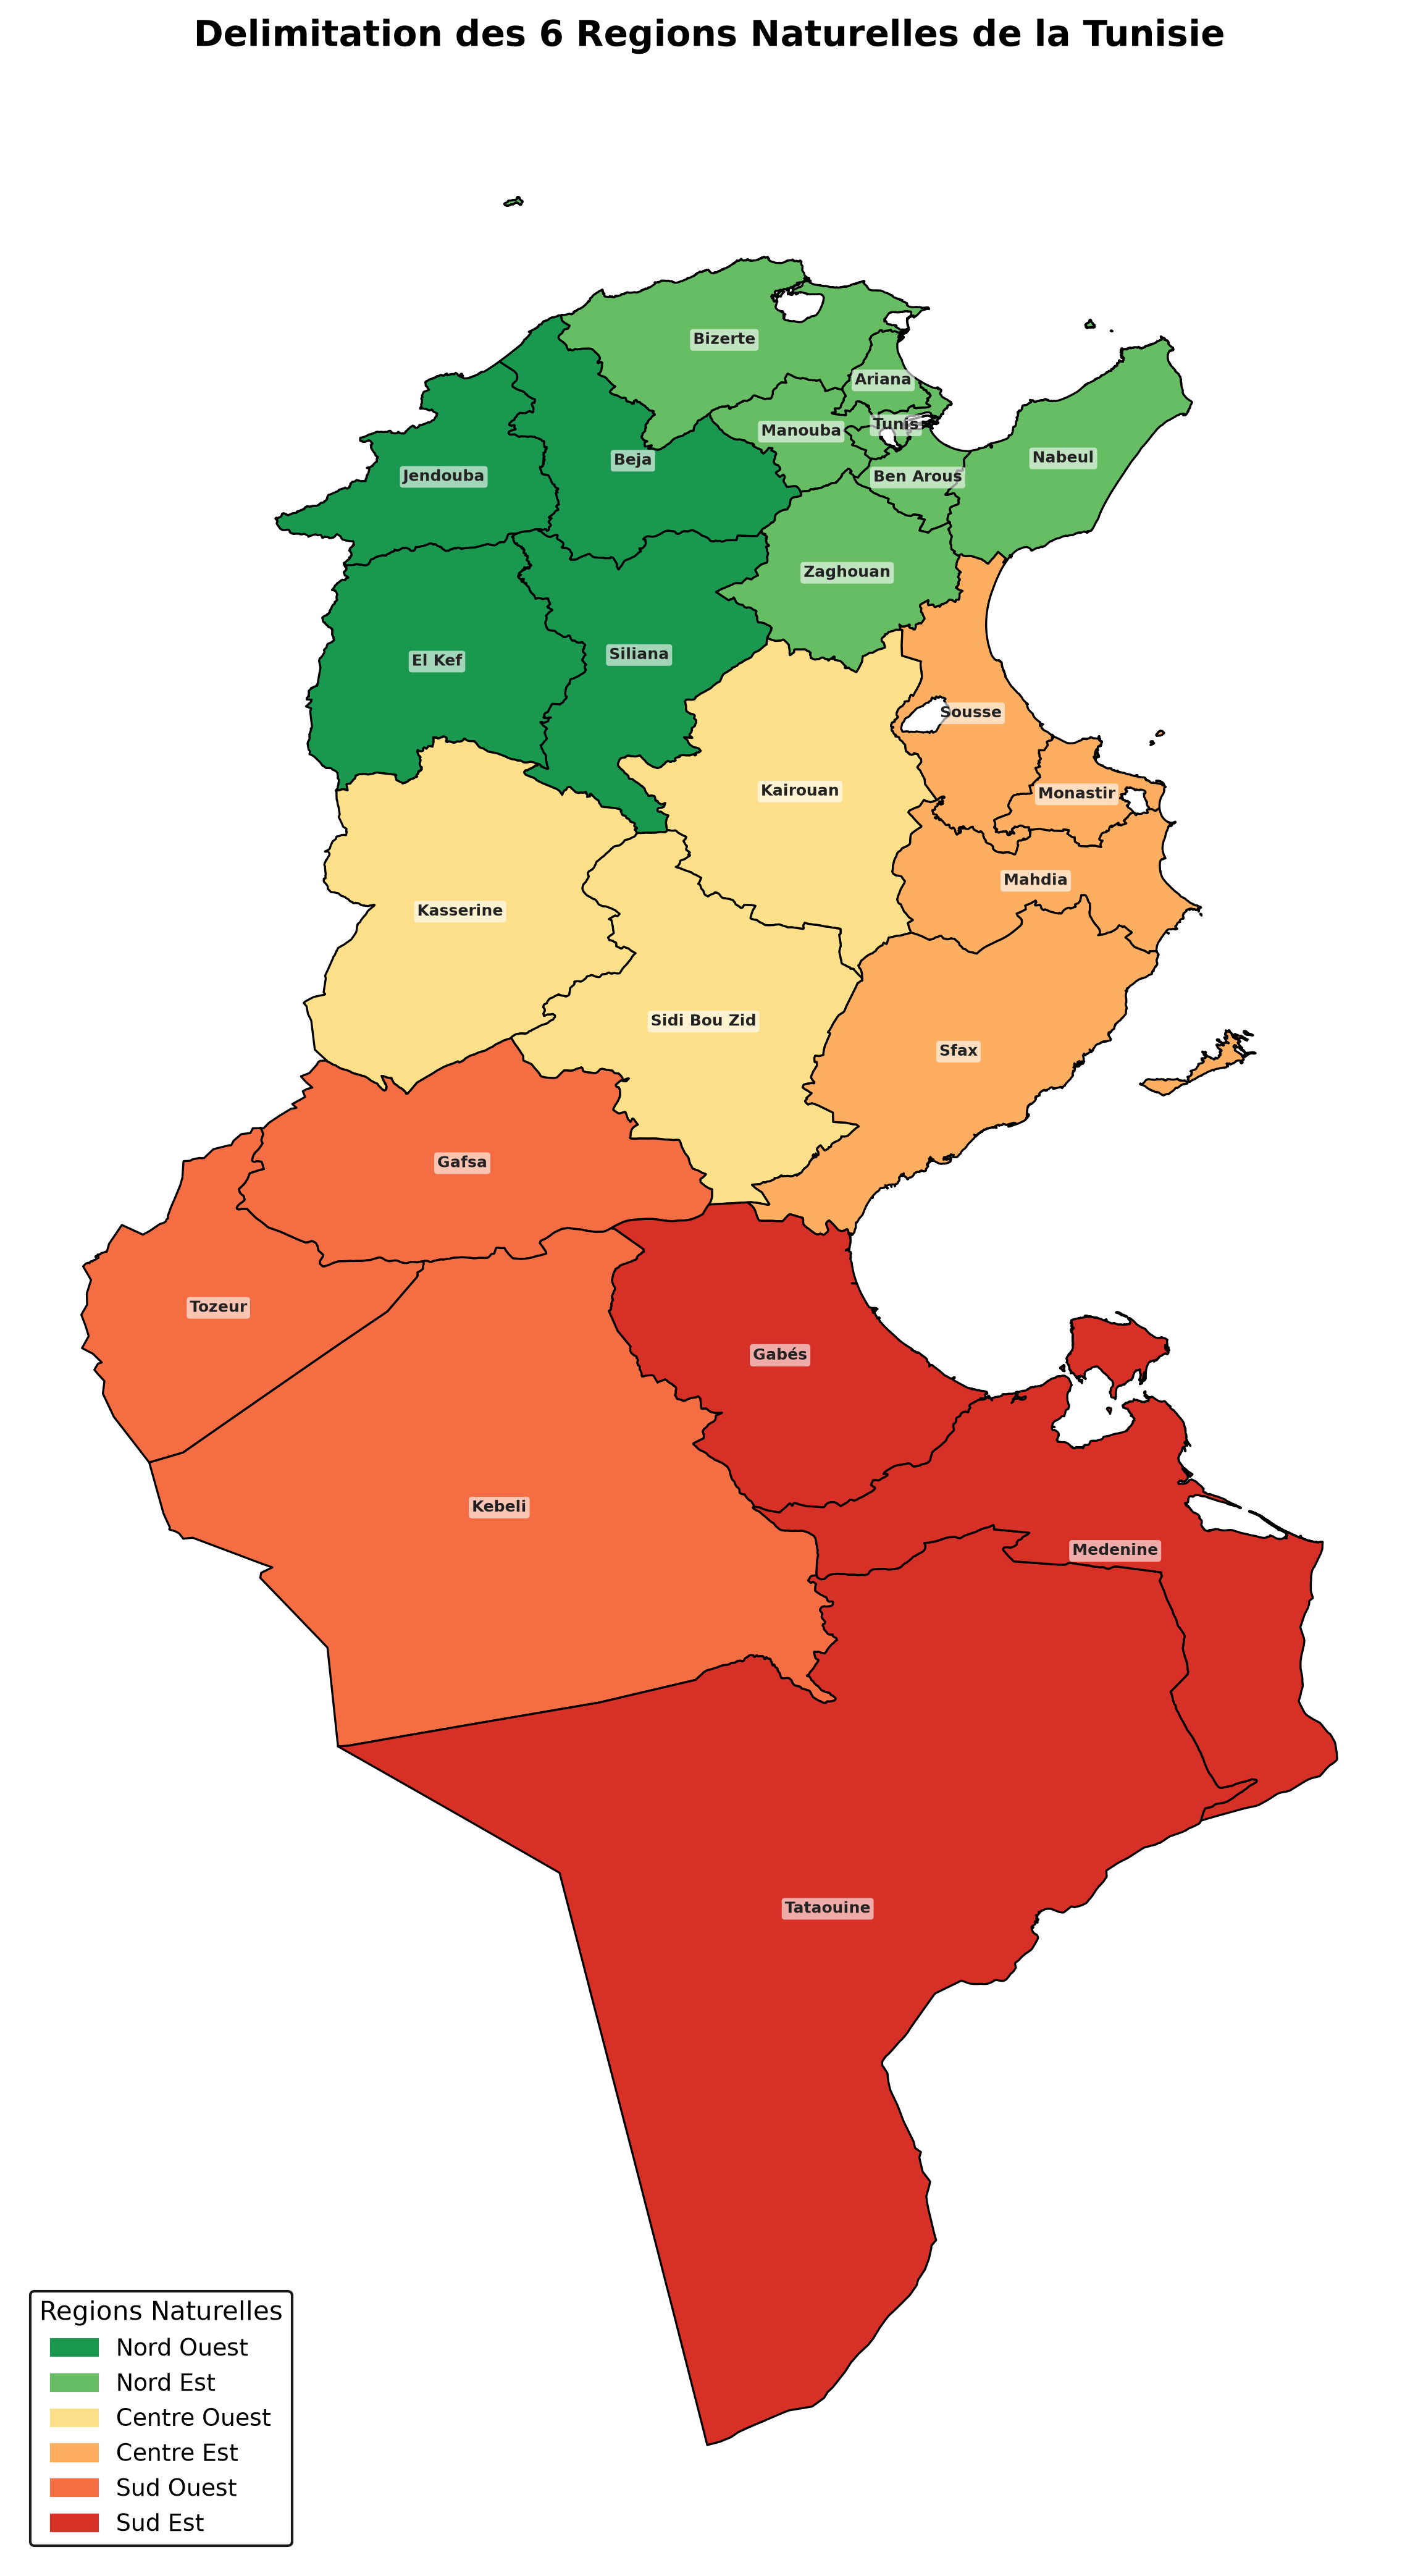
\includegraphics[width=0.68\textwidth]{figures/regions_naturelles_tunisie.png}
    \caption{The six Natural Regions of Tunisia utilized by the DGRE for regional water balance and weighted precipitation computations.}
    \label{fig:regions_naturelles}
\end{figure}

\begin{table}[htbp]
\centering
\caption{Characteristics of the six Natural Regions of Tunisia \cite{dgre2023}}
\label{tab:regions}
\small
\begin{tabular}{lrlc}
\toprule
\textbf{Natural Region} & \textbf{Area ($\text{km}^2$)} & \textbf{Governorates Included} & \textbf{Mean Annual Rain (mm)} \\
\midrule
Nord Ouest & 16,517 & Jendouba, Béja, Le Kef, Siliana & 500 -- 1200 \\
Nord Est & 11,725 & Tunis, Ariana, Ben Arous, Manouba, Nabeul, Zaghouan, Bizerte & 400 -- 650 \\
Centre Ouest & 22,184 & Kairouan, Kasserine, Sidi Bouzid & 200 -- 350 \\
Centre Est & 13,430 & Sousse, Monastir, Mahdia, Sfax & 250 -- 400 \\
Sud Ouest & 35,761 & Gafsa, Tozeur, Kébili & 80 -- 180 \\
Sud Est & 55,305 & Gabès, Tataouine, Médenine & 50 -- 150 \\
\midrule
\textbf{Total Tunisia} & \textbf{154,922} & \textbf{24 Governorates} & \textbf{National Avg: $\sim$216} \\
\bottomrule
\end{tabular}
\end{table}

\section{The Official Pluviometric Yearbook (*Annuaire Pluviométrique*)}

The \textit{Annuaire Pluviométrique de la Tunisie} is published for every hydrological year, which runs continuously from **September 1st of year $Y$ to August 31st of year $Y+1$**. This calendar ensures that winter precipitation is analyzed within a single continuous agricultural cycle. The official yearbook comprises three major elements:

\begin{enumerate}
  \item \textbf{Statistical Summary Tables}: A set of 8 standardized analytical tables:
  \begin{itemize}
    \item \textit{Tableau 1}: Regional synthesis comparing observed rainfall against interannual normals, calculating percentage ratios and deficits.
    \item \textit{Tableau 2}: Historical comparison across the preceding 8 hydrological years.
    \item \textit{Tableau 3}: Monthly precipitation totals by station and governorate.
    \item \textit{Tableau 4}: Seasonal aggregations (Autumn: Sep--Nov, Winter: Dec--Feb, Spring: Mar--May, Summer: Jun--Aug).
    \item \textit{Tableau 5}: Monthly and annual average precipitation by governorate.
    \item \textit{Tableau 6}: Detailed daily rainfall records for all 148 stations across 365 days.
    \item \textit{Tableau 7}: Cumulative rainfall progression curves month by month.
    \item \textit{Tableau 8}: Number of rainy days exceeding the significant 1.0~mm threshold.
  \end{itemize}
  \item \textbf{Cartographic Atlas}: A collection of 22 high-resolution isohyet maps:
  \begin{itemize}
    \item 1 Annual national isohyet map.
    \item 12 Monthly national isohyet maps.
    \item 4 Seasonal national isohyet maps.
    \item 1 Interannual 50-year normal isohyet map (1959--2009).
    \item 1 Ratio-to-normal anomaly map (percentage of long-term average).
    \item 3 Regional comparative hypsometric charts (North, Central, South).
  \end{itemize}
  \item \textbf{Hydrological Commentary}: Official narrative evaluating water reserves, drought intensity, and recharge implications.
\end{enumerate}

\section{Diagnosis of the Legacy Manual Workflow}

Figure~\ref{fig:current_workflow} illustrates the legacy procedural pipeline that historically governed yearbook generation at the DGRE.

\begin{figure}[htbp]
\centering
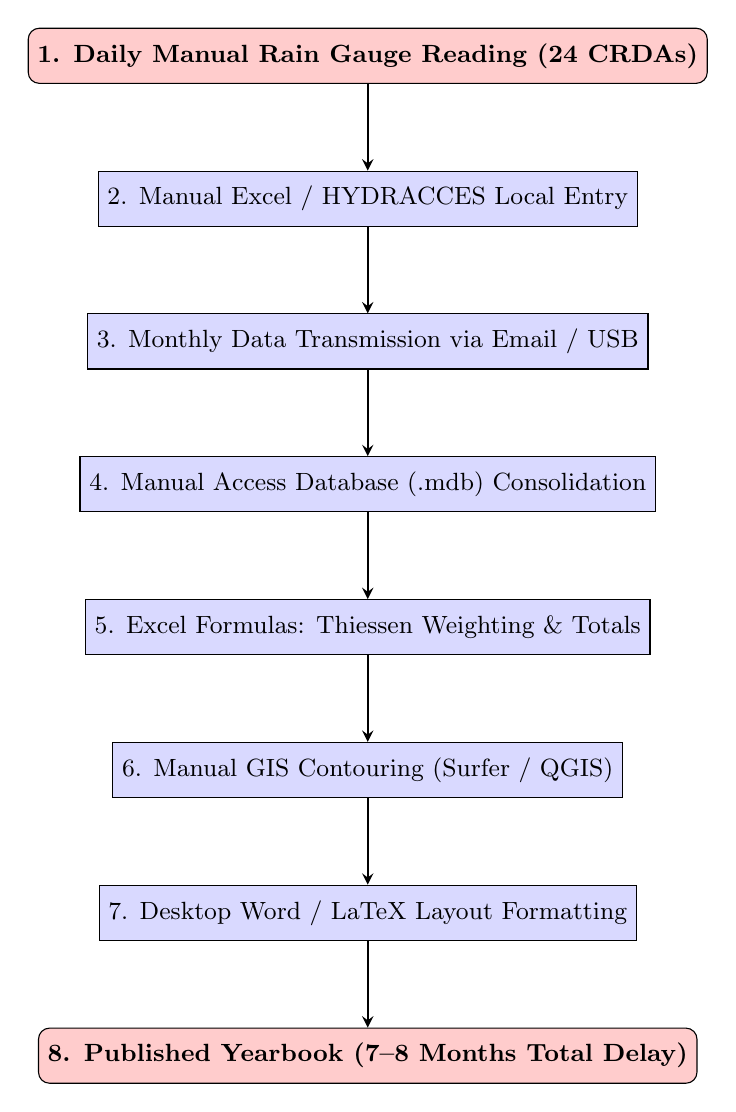
\begin{tikzpicture}[
  node distance=1.1cm,
  startstop/.style={rectangle, rounded corners, minimum width=3.5cm, minimum height=0.7cm, text centered, draw=black, fill=red!20, font=\small\bfseries},
  process/.style={rectangle, minimum width=5cm, minimum height=0.7cm, text centered, draw=black, fill=blue!15, font=\small},
  arrow/.style={thick,->,>=stealth}
]
\node (start) [startstop] {1. Daily Manual Rain Gauge Reading (24 CRDAs)};
\node (p1) [process, below=of start] {2. Manual Excel / HYDRACCES Local Entry};
\node (p2) [process, below=of p1] {3. Monthly Data Transmission via Email / USB};
\node (p3) [process, below=of p2] {4. Manual Access Database (.mdb) Consolidation};
\node (p4) [process, below=of p3] {5. Excel Formulas: Thiessen Weighting \& Totals};
\node (p5) [process, below=of p4] {6. Manual GIS Contouring (Surfer / QGIS)};
\node (p6) [process, below=of p5] {7. Desktop Word / LaTeX Layout Formatting};
\node (stop) [startstop, below=of p6] {8. Published Yearbook (7--8 Months Total Delay)};

\draw [arrow] (start) -- (p1);
\draw [arrow] (p1) -- (p2);
\draw [arrow] (p2) -- (p3);
\draw [arrow] (p3) -- (p4);
\draw [arrow] (p4) -- (p5);
\draw [arrow] (p5) -- (p6);
\draw [arrow] (p6) -- (stop);
\end{tikzpicture}
\caption{Legacy manual workflow for pluviometric yearbook compilation at the DGRE.}
\label{fig:current_workflow}
\end{figure}

The diagnostic assessment conducted during the initial phase of this internship revealed critical bottlenecks in this workflow:
\begin{itemize}
  \item \textbf{Data Sifting and Format Heterogeneity}: Each CRDA formatted its monthly submissions with subtle variations in station identifiers, accented characters, and date formats. Central technicians spent weeks reconciling records before ingestion.
  \item \textbf{Database Concurrency Failures}: Microsoft Access locks entire files during writes and lacks network concurrency, preventing multiple technicians from verifying regional data simultaneously.
  \item \textbf{Manual Spatial Interpolation}: Creating 22 isohyet maps required importing coordinate files into third-party desktop GIS packages, setting contour levels by hand, and manually exporting image files for document assembly.
  \item \textbf{Error Propagation}: A single updated rainfall measurement required manual re-computation of Excel sheets, re-export of spatial contour maps, and manual re-entry into the publication document.
\end{itemize}

These findings established the urgent institutional necessity for an integrated, automated platform combining spatial databases, mathematical algorithms, and artificial intelligence.

\newpage

% =====================================================================
% CHAPTER II: LITERATURE REVIEW & THEORETICAL FOUNDATIONS
% =====================================================================
\chapter{Literature Review and Theoretical Foundations}

\section{Introduction}

This chapter establishes the theoretical and methodological foundations of the Rainfull Cartagen platform. It examines Knowledge Management (KM) models applied to public natural resource governance, reviews the Design Thinking innovation framework, analyzes the mathematical formulations of spatial interpolation and integration (IDW vs. Thiessen), and surveys modern AI architectures including Multi-Agent systems, Retrieval-Augmented Generation (RAG), and defensive code sandboxing.

\section{Knowledge Management in Public Natural Resource Governance}

Knowledge Management (KM) is the systematic discipline of identifying, capturing, structuring, analyzing, and disseminating an institution's collective knowledge assets to enhance decision-making \cite{davenport1998, alavi2001}. In public institutions managing scarce natural resources, such as the DGRE, effective KM is vital to prevent institutional amnesia and ensure environmental resilience.

\subsection{The Knowledge Hierarchy: Data to Wisdom}
Tuomi \cite{tuomi1999} established that knowledge does not spontaneously arise from raw data; rather, raw data can only be captured once an underlying cognitive framework of knowledge already exists. Building upon the foundational KM literature \cite{davenport1998, king2005}, organizational assets operate across a four-tiered hierarchy:
\begin{itemize}
  \item \textbf{Data}: Unprocessed physical observations, such as raw rain gauge sensor values ($12.4\text{ mm}$ recorded at Station 102 on October 14th).
  \item \textbf{Information}: Data organized with contextual significance \cite{davenport1998}, including monthly aggregations, governorate totals, and station metadata.
  \item \textbf{Knowledge}: Actionable insights synthesized through human expertise and analytical models \cite{nonaka1994}, such as regional deficit percentages, spatial drought anomalies, and 50-year norm deviations.
  \item \textbf{Wisdom}: Strategic policy decisions informed by accumulated knowledge \cite{king2005}, including inter-basin water transfers, reservoir discharge scheduling, and emergency drought declarations.
\end{itemize}

Rainfull Cartagen acts as an automated cognitive bridge transforming raw daily rainfall \textit{data} into structured \textit{information} and spatial \textit{knowledge}, enabling strategic institutional \textit{wisdom}.

\subsection{Nonaka and Takeuchi's SECI Model Applied to the DGRE}
Nonaka and Takeuchi's SECI model \cite{nonaka1995} articulates how knowledge converts between tacit (implicit human experience) and explicit (codified) forms through four dynamic quadrants \cite{nonaka1994}:
\begin{enumerate}
  \item \textbf{Socialization (Tacit $\rightarrow$ Tacit)}: Senior DGRE hydrologists mentoring junior technicians on identifying anomalous gauge readings caused by wind drift or debris blockage.
  \item \textbf{Externalization (Tacit $\rightarrow$ Explicit)}: Codifying the empirical rules, Thiessen boundary adjustments, and contour smoothing guidelines into explicit Python algorithms and formal software architecture.
  \item \textbf{Combination (Explicit $\rightarrow$ Explicit)}: Integrating disparate rainfall files from 24 CRDAs with digital spatial boundaries and historical norm tables into a unified PostGIS database and automated yearbook.
  \item \textbf{Internalization (Explicit $\rightarrow$ Tacit)}: Technicians and decision-makers analyzing the automatically generated anomaly maps and agent reasoning traces, absorbing new spatial patterns of national climate vulnerability.
\end{enumerate}

\subsection{Knowledge Management Life Cycles}
The theoretical literature identifies several integrated KM cycle models:
\begin{itemize}
  \item \textbf{Meyer and Zack Model (1996)}: Focuses on the production of ``information products'' through five stages: \textit{Acquisition}, \textit{Refinement}, \textit{Storage/Retrieval}, \textit{Distribution}, and \textit{Presentation} \cite{meyer1996}. Rainfull Cartagen directly operationalizes this cycle: ingesting CRDA files (Acquisition), calculating Thiessen and IDW indicators (Refinement), archiving in PostGIS and Zvec (Storage), serving via FastAPI (Distribution), and rendering PDF yearbooks (Presentation).
  \item \textbf{Dalkir's Integrated KM Life Cycle (2017)}: Synthesizes earlier frameworks into three integrated phases: \textit{Knowledge Creation/Capture}, \textit{Knowledge Sharing/Dissemination}, and \textit{Knowledge Acquisition/Application} \cite{dalkir2017}. Dalkir emphasizes continuous quality assessment during transitions, mirror-imaged in Rainfull Cartagen by the Quality Verification Agent's validation loops.
  \item \textbf{Bukowitz and Williams Framework (2000)}: Explores strategic tactical cycles where organizations \textit{Get}, \textit{Use}, \textit{Learn}, and \textit{Contribute} knowledge assets to maintain competitive capability \cite{bukowitz2000}.
  \item \textbf{Wiig's KM Cycle (1993)}: Emphasizes that knowledge must be made actionable through \textit{Creation}, \textit{Sourcing}, \textit{Compilation}, \textit{Transformation}, and \textit{Application} \cite{wiig1993}.
\end{itemize}

\subsection{Organizational Memory and Knowledge Transfer}
Huber \cite{huber1991} defines organizational memory as the means through which knowledge from past actions and events is preserved to inform current behaviors. Cross and Baird \cite{cross2000} emphasize that technology alone is insufficient; memory must reside in structured repositories that survive organizational turnover. As veteran hydrologists retire from the DGRE, Rainfull Cartagen ensures that institutional expertise remains actively executable in production code rather than being lost \cite{argote2000}.

\section{Methodological Framework: Design Thinking}

To ensure that the engineered software matched the exact operational practices of the DGRE, the project adopted the \textbf{Design Thinking} methodology formalized by Brown \cite{brown2009} and Koskinen \cite{koskinen2018}. The three core phases guided implementation:
\begin{enumerate}
  \item \textbf{Inspiration}: Immersing in the daily routines of the \textit{Sous-Direction de l'Hydrologie Analytique}, conducting stakeholder interviews with technicians, database administrators, and directors, and observing manual data entry bottlenecks.
  \item \textbf{Ideation}: Brainstorming architectural alternatives to address the core problem: ``How might we compress an 8-month manual publication process into an instantaneous, reproducible automated workflow?''
  \item \textbf{Implementation}: Iterative prototyping of PostgreSQL schemas, Python calculation modules, multi-agent prompts, and user interfaces, with weekly validation sessions alongside DGRE practitioners acting as \textit{Lead Users} \cite{vonhippel1986}.
\end{enumerate}

\section{Spatial Statistics and Hydrological Interpolation}

Rainfall measured at discrete point stations must be converted into spatial continuous surfaces and aggregate regional indices. Two distinct mathematical methodologies are employed by the DGRE.

\subsection{The Thiessen Polygon Method (Voronoi Tessellation)}
The Thiessen polygon method \cite{thiessen1911} is the official standard mandated by the DGRE for computing regional and national mean precipitation ($P_R$). Given a set of $N$ monitoring stations within region $R$, the planar space is decomposed into Voronoi polygons $V_i$, where every point inside polygon $V_i$ is geographically closer to station $i$ than to any other station:
\begin{equation}
V_i = \left\{ (x, y) \in R \;\middle|\; \|(x,y) - (x_i, y_i)\| \leq \|(x,y) - (x_j, y_j)\|, \;\forall j \neq i \right\}
\label{eq:voronoi}
\end{equation}

The surface area of each clipped polygon within region $R$ is denoted $A_i^R$. The surface weighting coefficient $w_i^R$ allocated to station $i$ is:
\begin{equation}
w_i^R = \frac{A_i^R}{\sum_{j=1}^{N} A_j^R} = \frac{A_i^R}{A_R}, \quad \text{with } \sum_{i=1}^{N} w_i^R = 1
\label{eq:thiessen_weight}
\end{equation}

The regional average rainfall $P_R$ is subsequently obtained via discrete spatial integration:
\begin{equation}
P_R = \sum_{i=1}^{N} w_i^R \cdot P_i
\label{eq:thiessen_mean}
\end{equation}
where $P_i$ represents the cumulative precipitation measured at station $i$. Thiessen polygons provide an objective, mathematically rigorous area-weighted average that accounts for uneven station density.

\subsection{Inverse Distance Weighting (IDW) Continuous Interpolation}
While Thiessen polygons produce discrete stair-step averages, visualizing precipitation gradients requires a continuous spatial field $Z(x, y)$ to draw smooth isohyet contours. The DGRE adopts Inverse Distance Weighting (IDW) interpolation \cite{shepard1968}.

For any target point $p = (x, y)$ on a regular grid, the estimated precipitation $Z(p)$ is a weighted average of observed station values $Z_i = Z(s_i)$:
\begin{equation}
Z(p) = \frac{\sum_{i=1}^{K} \omega_i(p) \cdot Z_i}{\sum_{i=1}^{K} \omega_i(p)}
\label{eq:idw_formula}
\end{equation}
where the weight $\omega_i(p)$ is inversely proportional to the Euclidean distance $d(p, s_i)$ raised to power $\alpha$:
\begin{equation}
\omega_i(p) = \frac{1}{d(p, s_i)^\alpha} = \frac{1}{\left( \sqrt{(x - x_i)^2 + (y - y_i)^2} + \epsilon \right)^\alpha}
\label{eq:idw_weights}
\end{equation}
In accordance with DGRE cartographic standards, the power exponent is calibrated to $\alpha = 2.0$ (gravity-based attenuation), and a smoothing factor $\epsilon = 0.5\text{ m}$ is introduced to prevent division by zero when evaluating grid points directly atop a station marker.

\begin{figure}[htbp]
    \centering
    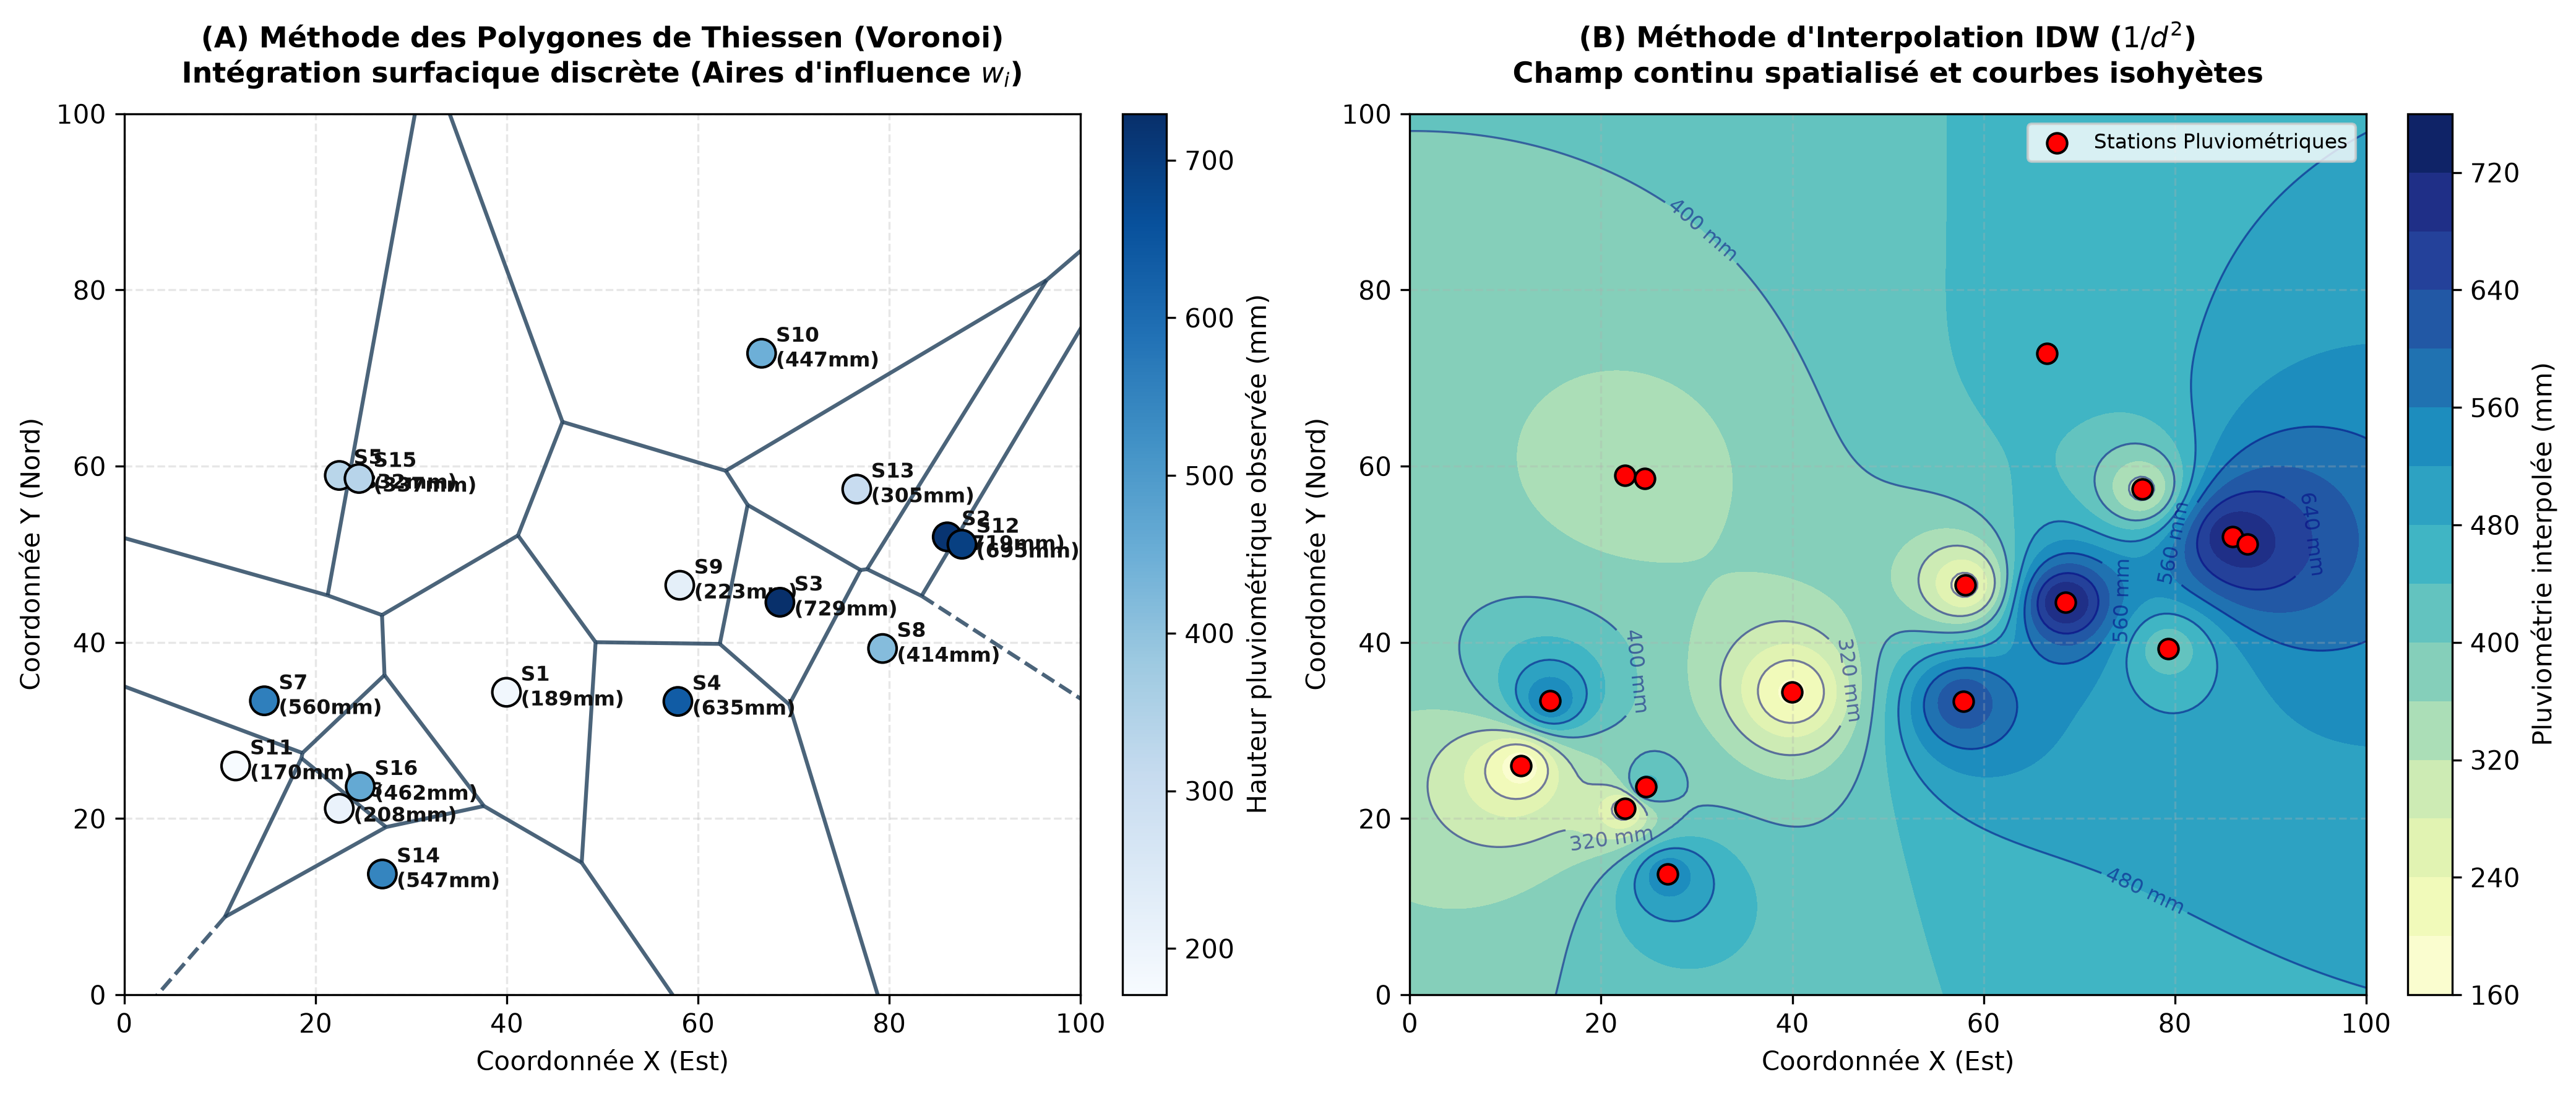
\includegraphics[width=0.92\textwidth]{figures/comparaison_thiessen_idw.png}
    \caption{Methodological comparison between discrete surface integration via Thiessen Polygons (left) and continuous spatial gradient interpolation via IDW (right).}
    \label{fig:thiessen_vs_idw}
\end{figure}

Figure~\ref{fig:thiessen_vs_idw} highlights the complementary roles of both methods: Thiessen polygons discretize the territory into distinct administrative and regional catchment areas to populate statistical tables, while IDW computes smooth 2D raster surfaces for isohyet contouring.

\section{Artificial Intelligence, Multi-Agent Systems, and Security}

\subsection{Supervisor Multi-Agent Pattern}
Modern Large Language Models (LLMs) excel at natural language parsing but struggle with complex, multi-step domain workflows when prompted as monolithic systems. Rainfull Cartagen implements the \textbf{Supervisor Pattern} \cite{wooldridge2009}, wherein an autonomous orchestrator decomposes user requests into specialized sub-tasks assigned to dedicated functional agents communicating across a structured message bus.

\subsection{Retrieval-Augmented Generation (RAG)}
To eliminate hallucination risks and provide LLMs with dynamic domain context without costly full model retraining, the platform employs Retrieval-Augmented Generation (RAG) \cite{lewis2020}. By indexing historical rainfall summaries, station catalogs, and verified GIS code snippets into a dense vector space, relevant context is retrieved via cosine similarity and injected into the prompt before generation.

\subsection{Parameter-Efficient Fine-Tuning (PEFT / LoRA)}
To specialize smaller open-source models (such as Llama-3.1-8B) for domain-specific SQL generation and geospatial script authoring, Low-Rank Adaptation (LoRA) \cite{hu2021} is applied. LoRA freezes the original model parameters $W_0 \in \mathbb{R}^{d \times k}$ and introduces low-rank trainable decomposition matrices $A \in \mathbb{R}^{r \times k}$ and $B \in \mathbb{R}^{d \times r}$ with rank $r \ll \min(d, k)$:
\begin{equation}
W = W_0 + \Delta W = W_0 + \frac{\alpha}{r} (B \cdot A)
\label{eq:lora}
\end{equation}
This allows training the model on consumer GPUs while drastically reducing parameter count and preventing catastrophic forgetting.

\subsection{Defensive Sandboxing and AST Validation}
Allowing an LLM to generate and execute Python code dynamically introduces severe security risks, including arbitrary code execution and system tampering \cite{owasp2024}. Rainfull Cartagen addresses this through a multi-tier defense: static code analysis via Python's Abstract Syntax Tree (\texttt{ast}) module blocking forbidden system calls prior to execution, combined with isolated subprocess sandboxing under strict timeouts.

\newpage

% =====================================================================
% CHAPTER III: SYSTEM ANALYSIS, MODELING & ARCHITECTURE
% =====================================================================
\chapter{System Analysis, Modeling, and Architecture}

\section{Introduction}

This chapter details the engineering design of the Rainfull Cartagen platform. It formalizes user requirements, presents the conceptual and physical database modeling following the MERISE methodology, details the database migration to PostgreSQL/PostGIS, outlines the Clean/Hexagonal multi-agent architecture, explains the mathematical implementation of hydrological algorithms, and details the defensive security sandbox.

\section{Requirements Analysis}

Following the Design Thinking stakeholder analysis at the DGRE, the system requirements were formalized into functional and non-functional specifications.

\subsection{Functional Specifications}
\begin{itemize}
  \item \textbf{FS-01 (Data Migration \& Management)}: Ingest and consolidate legacy MS Access (.mdb) files, station catalogues, and shapefiles into a centralized, queryable relational repository with full CRUD capabilities.
  \item \textbf{FS-02 (Statistical Computation Engine)}: Automatically calculate all 8 official yearbook tables (Tableaux 1 to 8), including monthly totals, cumulative sums, rainy days ($\geq 1\text{ mm}$), and Thiessen-weighted regional averages.
  \item \textbf{FS-03 (Automated Cartographic Synthesis)}: Generate 22 high-resolution (300 DPI) maps (annual, monthly, seasonal, normal, anomaly) in UTM Zone 32N with official DGRE color legends, scale bars, and north arrows.
  \item \textbf{FS-04 (Multi-Agent Conversational Interface)}: Provide a web chat interface allowing users to query rainfall data in natural French or English and receive analytical text, statistical tables, or dynamic isohyet maps.
  \item \textbf{FS-05 (Instantaneous PDF Yearbook Assembly)}: Dynamically assemble and compile the complete, publication-ready annual yearbook in PDF format via automated LaTeX compilation in under 5 minutes.
\end{itemize}

\subsection{Non-Functional Specifications}
\begin{itemize}
  \item \textbf{NFS-01 (Mathematical Parity)}: Zero numerical discrepancy against official DGRE historical yearbooks (tolerance $< 0.1\text{ mm}$).
  \item \textbf{NFS-02 (Execution Security)}: 100\% interception of malicious or destructive code generated by AI models via AST validation and isolated sandboxing.
  \item \textbf{NFS-03 (Modularity \& Maintainability)}: Decoupled Clean Architecture ensuring that LLM providers or database backends can be swapped without rewriting core business logic.
  \item \textbf{NFS-04 (On-Premises Deployability)}: Fully containerized deployment using Docker Compose operating within the closed DGRE intranet without external cloud dependencies.
\end{itemize}

\section{Database Conceptual Modeling and Migration}

\subsection{MERISE Conceptual Data Model (MCD)}
The conceptual design of the spatialized repository was formulated using the MERISE methodology \cite{baptiste2024}. The core entities and relationships are:
\begin{itemize}
  \item \textbf{STATION}: Identified by \texttt{id\_station}, storing official name, governorate, coordinates ($X, Y$ in UTM 32N), and altitude.
  \item \textbf{OBSERVATION\_PLUIE}: Weak entity linked to \textbf{STATION}, recording daily precipitation values (\texttt{valeur\_mm}) on specific timestamps (\texttt{date\_obs}).
  \item \textbf{MOY\_INTERANNUELLE}: Stores the 50-year historical normal (1959--2009) associated with each reference station.
  \item \textbf{GOUVERNORAT} \& \textbf{REGION\_NATURELLE}: Represent spatial administrative and natural boundaries, holding multipolygon geometries.
\end{itemize}

The cardinalities governing the entities are summarized in Table~\ref{tab:cardinalities}.

\begin{table}[htbp]
\centering
\caption{MERISE Entity-Relationship cardinalities for the Rainfull Cartagen database}
\label{tab:cardinalities}
\small
\begin{tabular}{lllp{6cm}}
\toprule
\textbf{Entity 1} & \textbf{Relationship} & \textbf{Entity 2} & \textbf{Cardinality \& Description} \\
\midrule
STATION & Mesure & OBSERVATION\_PLUIE & $1,1 \longleftrightarrow 0,N$ (A station records zero or many daily observations; each observation belongs to exactly one station). \\
STATION & Possède & MOY\_INTERANNUELLE & $1,1 \longleftrightarrow 1,1$ (Each reference station possesses exactly one 50-year interannual average). \\
GOUVERNORAT & Contient & STATION & $1,N \longleftrightarrow 1,1$ (A governorate contains one or more stations; a station belongs to one governorate). \\
REGION\_NAT & Englobe & GOUVERNORAT & $1,N \longleftrightarrow 1,1$ (A natural region encompasses multiple governorates). \\
\bottomrule
\end{tabular}
\end{table}

\subsection{Database Migration: MS Access to PostgreSQL/PostGIS}
Table~\ref{tab:db_comparison} contrasts the legacy Microsoft Access system against the newly deployed PostgreSQL/PostGIS spatial architecture \cite{stonebraker2018, postgresql2024, postgis2024}.

\begin{table}[htbp]
\centering
\caption{Architectural comparison between legacy MS Access and PostgreSQL/PostGIS}
\label{tab:db_comparison}
\small
\begin{tabular}{p{3.5cm}p{5.5cm}p{5.5cm}}
\toprule
\textbf{Dimension} & \textbf{Legacy MS Access (.mdb)} & \textbf{Deployed PostgreSQL/PostGIS} \\
\midrule
\textbf{Geospatial Engine} & None (coordinates stored as text/floats; no spatial queries). & Native PostGIS geometry types (\texttt{Point}, \texttt{MultiPolygon}) with spatial indexing (GiST). \\
\textbf{Concurrency} & File-level locking; corrupts easily with $>3$ concurrent users. & Row-level locking (MVCC); supports hundreds of concurrent API connections. \\
\textbf{Coordinate Transforms} & Impossible; requires external desktop GIS software. & In-database on-the-fly transformations via \texttt{ST\_Transform()}. \\
\textbf{Volume \& Scale} & Maximum file size capped at 2~GB. & Unlimited multi-terabyte storage with table partitioning. \\
\textbf{Web Integration} & Unsuitable for web APIs or microservice architectures. & Native async drivers (asyncpg, SQLAlchemy) integrated with FastAPI. \\
\bottomrule
\end{tabular}
\end{table}

The physical relational schema deployed in the production database \texttt{dgre\_db} includes spatial tables indexed with GiST:
\begin{lstlisting}[style=sqlstyle, caption={Core relational schema of dgre\_db with PostGIS spatial indexing}]
CREATE EXTENSION IF NOT EXISTS postgis;

CREATE TABLE station_148 (
    id_station   BIGINT PRIMARY KEY,
    nom          VARCHAR(100) NOT NULL,
    gouvernorat  VARCHAR(50) NOT NULL,
    x            DOUBLE PRECISION NOT NULL, -- UTM 32N Easting (m)
    y            DOUBLE PRECISION NOT NULL, -- UTM 32N Northing (m)
    altitude     DOUBLE PRECISION,
    geom         GEOMETRY(Point, 32632)
);
CREATE INDEX idx_station_geom ON station_148 USING GIST (geom);

CREATE TABLE pluies_148 (
    id           BIGSERIAL PRIMARY KEY,
    id_station   BIGINT REFERENCES station_148(id_station),
    date_obs     DATE NOT NULL,
    valeur_mm    DOUBLE PRECISION NOT NULL
);
CREATE INDEX idx_pluies_date ON pluies_148 (date_obs);
CREATE INDEX idx_pluies_station ON pluies_148 (id_station);

CREATE TABLE moy_interannuelle (
    id_station   BIGINT PRIMARY KEY REFERENCES station_148(id_station),
    moy          DOUBLE PRECISION NOT NULL -- 50-year norm (mm)
);
\end{lstlisting}

\section{Multi-Agent System Architecture}

Rainfull Cartagen implements a modular \textbf{Clean Architecture} where domain logic and multi-agent coordination are decoupled from web delivery and database drivers.

\begin{figure}[htbp]
    \centering
    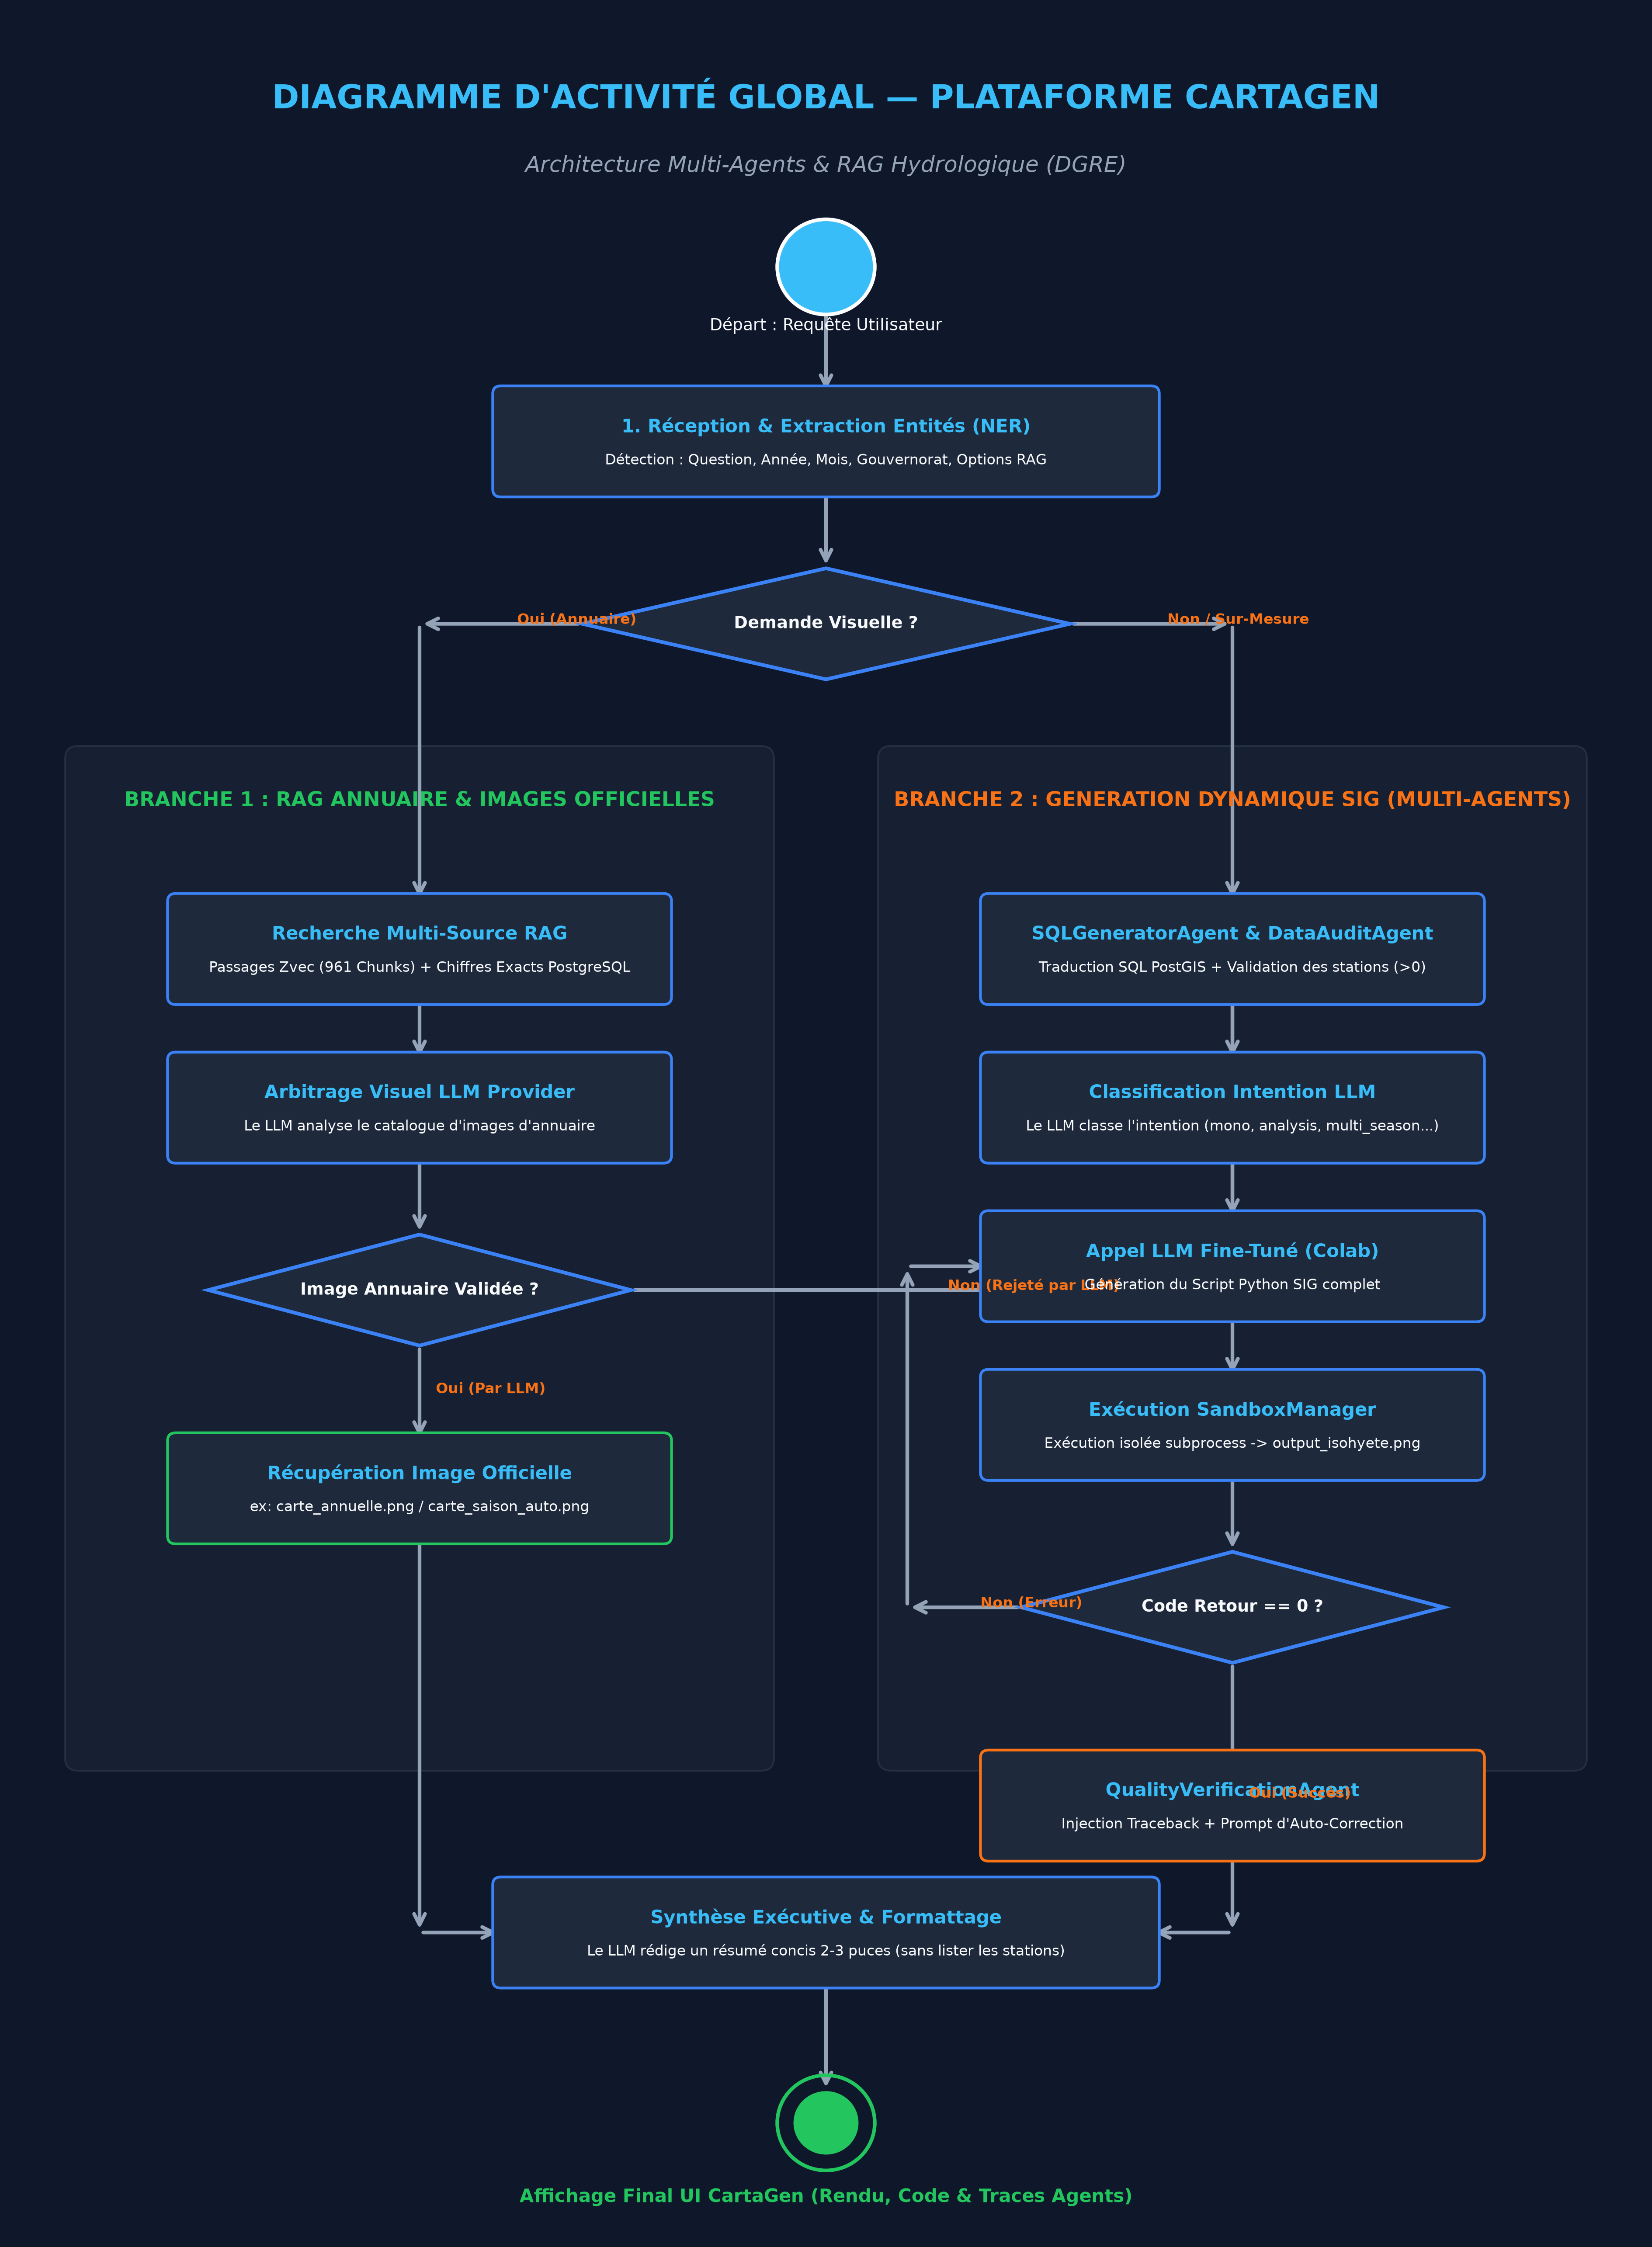
\includegraphics[width=0.88\textwidth]{figures/diagramme_activite_multiagents.png}
    \caption{UML activity diagram illustrating the multi-agent deliberation cycle, prompt tracing, and autonomous self-correction loop.}
    \label{fig:activite_multiagents}
\end{figure}

As shown in the activity diagram in Figure~\ref{fig:activite_multiagents}, user requests initiate a structured deliberation sequence:
\begin{enumerate}
  \item \textbf{CartaGenOrchestrator}: The central supervisor inspects the user prompt and performs semantic intent classification:
  \begin{itemize}
    \item \textit{Intent A (Data Query / Statistics)}: Dispatched to the \textbf{SQLGeneratorAgent}.
    \item \textit{Intent B (Map Synthesis / Cartography)}: Dispatched to the \textbf{SIGGeneratorAgent}.
    \item \textit{Intent C (Yearbook Question / Institutional Image)}: Dispatched to the \textbf{AnnuaireRAGAgent}.
    \item \textit{Intent D (Full Yearbook Generation)}: Triggers the automated LaTeX compiler pipeline.
  \end{itemize}
  \item \textbf{MessageBus with Real-Time Tracing}: All inter-agent communications, system prompts, raw LLM completions, and execution traces are logged in structured JSON format and pushed via WebSockets to the web dashboard.
  \item \textbf{SQLGeneratorAgent}: Translates natural language questions into sanitized SQL queries against the \texttt{dgre\_db} PostGIS database. It enforces table whitelisting and double-quotes user inputs to eliminate SQL injection vulnerabilities.
  \item \textbf{SIGGeneratorAgent}: Dynamically synthesizes executable Python scripts to generate custom cartography. Rather than generating scripts from scratch, it loads certified parameter-driven templates from the \texttt{skeletons/} repository (e.g., \texttt{isohyet\_contour.py.template}, \texttt{stations\_density.py.template}) using an LRU cache.
  \item \textbf{QualityVerificationAgent}: Acts as an automated code reviewer. When the Sandbox reports a non-zero exit code or stderr traceback, the Quality agent analyzes the error message, constructs a corrective prompt, and triggers an autonomous code repair loop (up to 3 iterative retries).
  \item \textbf{AnnuaireRAGAgent}: Integrates an in-process vector store (\textbf{Zvec}) containing 961 chunked passages of historical yearbooks. It employs an \textit{All-MiniLM-L6-v2} embedding model with HNSW cosine similarity search, applying a temporal filter on the requested year and a \textbf{+30\% spatial boost} for passages matching the queried governorate.
\end{enumerate}

\section{Defensive Security and Sandbox Architecture}

To provide complete isolation during the execution of AI-generated Python scripts, Rainfull Cartagen implements a two-stage security barrier, illustrated in Figure~\ref{fig:securite_sandbox}.

\begin{figure}[htbp]
    \centering
    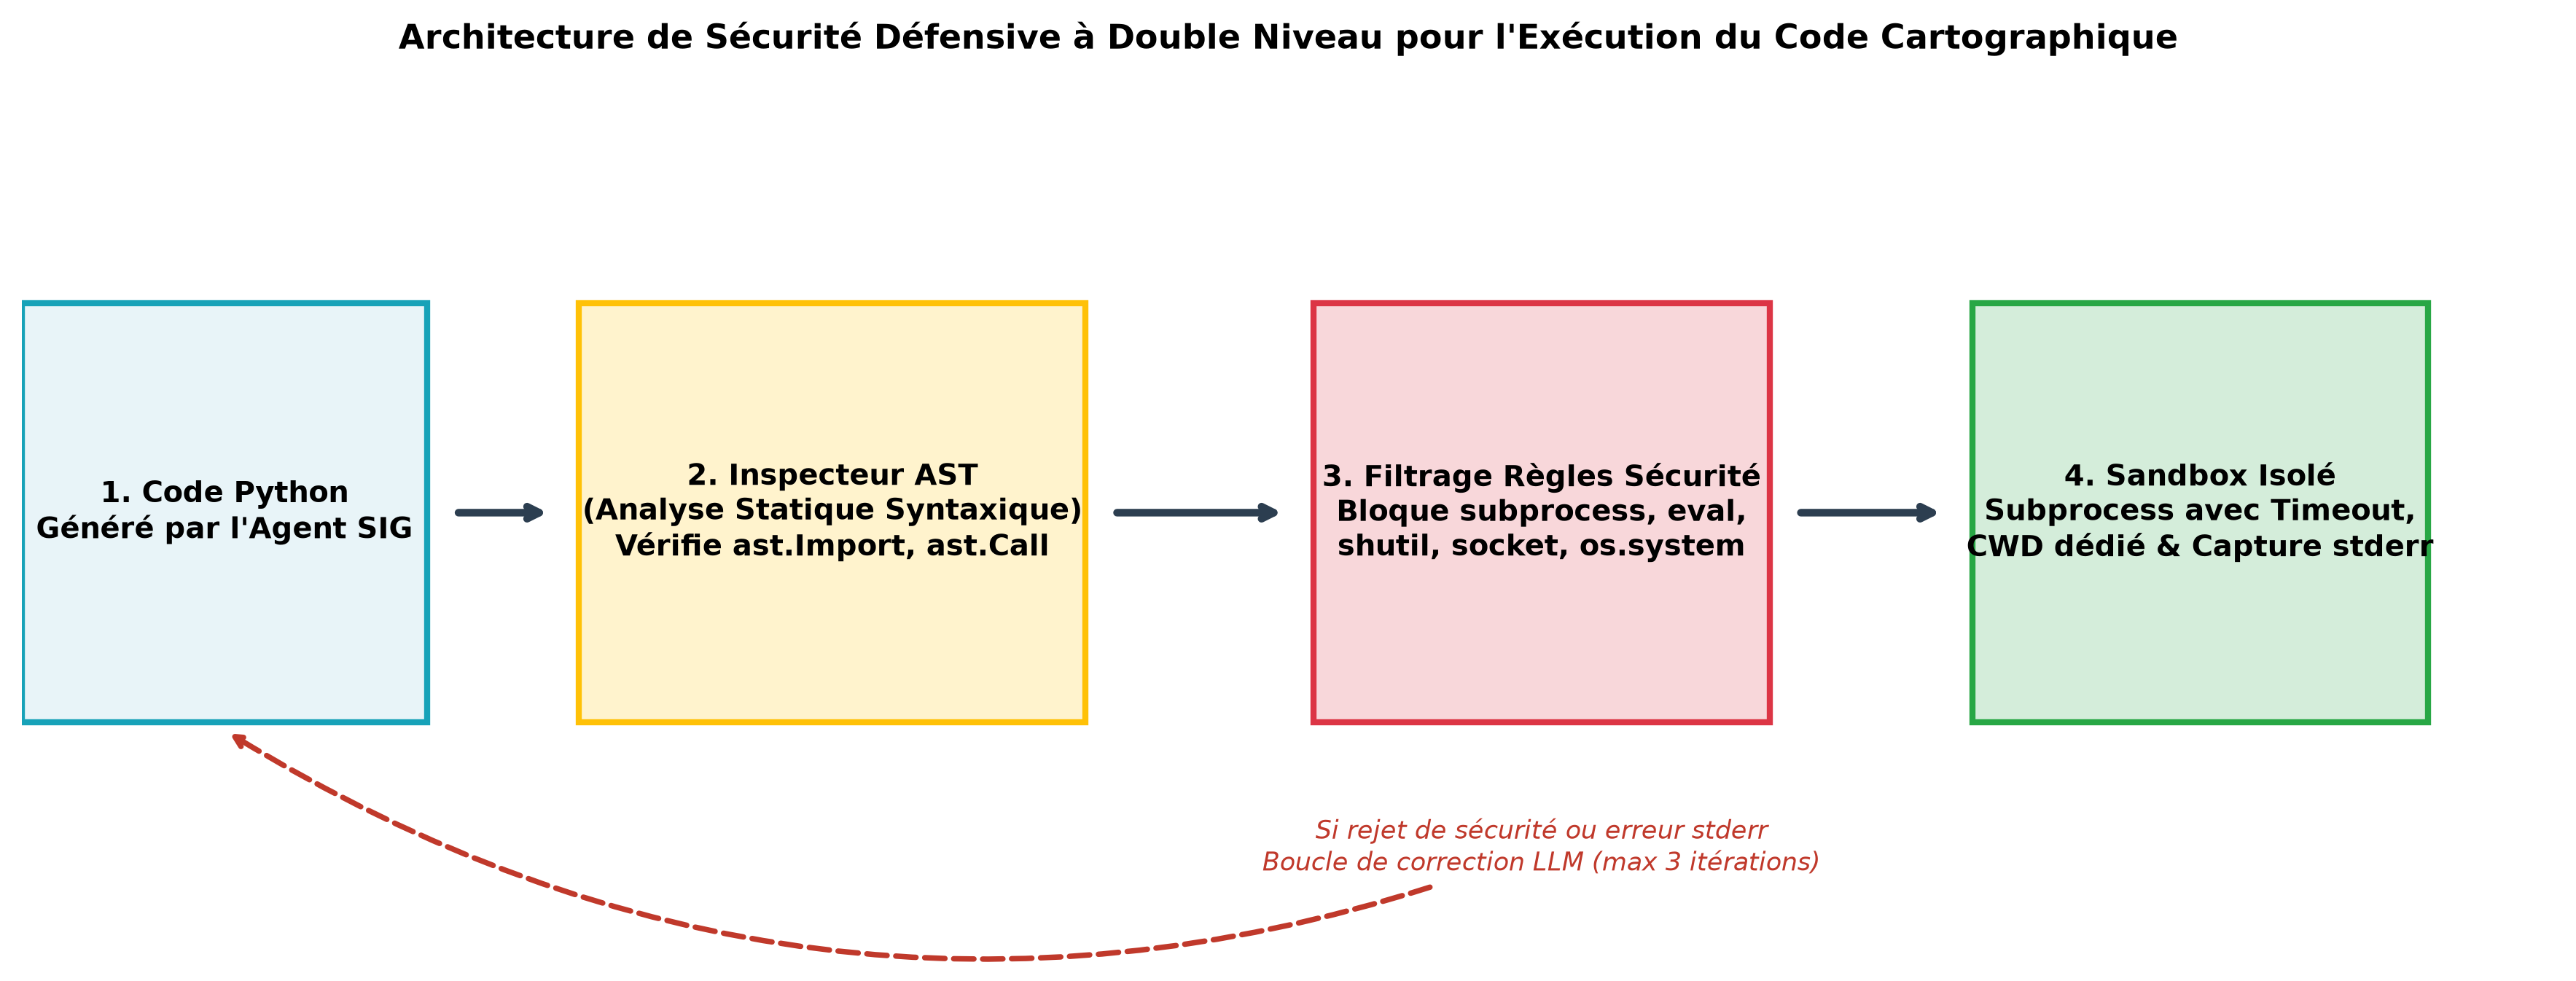
\includegraphics[width=0.92\textwidth]{figures/pipeline_securite_sandbox.png}
    \caption{Two-stage defensive security pipeline: static Abstract Syntax Tree (AST) validation followed by isolated subprocess sandboxing.}
    \label{fig:securite_sandbox}
\end{figure}

\subsection{Static AST Code Validation (\texttt{CodeSecurityValidator})}
Prior to invoking the Python runtime, the generated script is parsed into an Abstract Syntax Tree via Python's built-in \texttt{ast} library. The validator traverses the AST and immediately rejects any script that attempts to:
\begin{itemize}
  \item Import prohibited modules: \texttt{subprocess}, \texttt{shutil}, \texttt{socket}, \texttt{requests}, \texttt{urllib}, \texttt{ftplib}, \texttt{pty}, \texttt{sys}, or \texttt{importlib}.
  \item Invoke dangerous built-in functions: \texttt{eval()}, \texttt{exec()}, \texttt{compile()}, \texttt{open()} (in write/append mode outside sandbox), \texttt{getattr()}, or \texttt{\_\_import\_\_}.
  \item Execute shell commands via \texttt{os.system()}, \texttt{os.popen()}, \texttt{os.spawn*()}, or access private object attributes (\texttt{\_\_subclasses\_\_}, \texttt{\_\_globals\_\_}).
\end{itemize}

\subsection{Isolated Subprocess Sandbox (\texttt{SandboxManager})}
Once validated by the AST inspector, the script is written to a temporary sandboxed workspace (\texttt{sandbox\_runs/run\_<id>/}). Execution occurs within an isolated subprocess under stringent operational constraints:
\begin{itemize}
  \item Hard wall-clock execution timeout enforced at **30 seconds** (mitigating infinite loops or CPU exhaustion).
  \item Dedicated working directory preventing path traversal into parent source repositories.
  \item Complete capture and structured parsing of \texttt{stdout} and \texttt{stderr}.
\end{itemize}

\newpage

% =====================================================================
% CHAPTER IV: IMPLEMENTATION, EXPERIMENTAL RESULTS & DEPLOYMENT
% =====================================================================
\chapter{Implementation, Experimental Results, and Deployment}

\section{Introduction}

This chapter details the concrete implementation and operational achievements of Rainfull Cartagen. It synthesizes the development chronicle from the internship journal, details the AI fine-tuning and dataset balancing engineering, showcases the generated cartographic and tabular deliverables, validates mathematical parity against official DGRE records, and presents the containerized deployment architecture.

\section{Implementation Chronicle and Key Milestones}

The implementation was executed over a 7-week period at the DGRE (June 15 to July 30, 2026), documented in the official internship log (\textit{Journal de stage}):

\begin{itemize}
  \item \textbf{Week 1 (June 15 -- June 19)}: Orientation meeting with DGRE leadership. Data discovery and legacy Access database audit. Analysis of data anomalies in coordination with the DGRE data analysis team. Comparative benchmark of Python geospatial libraries (GeoPandas, Folium, Matplotlib, Cartopy).
  \item \textbf{Week 2 (June 22 -- June 26)}: Local environment setup. Initial cartographic prototyping. \textbf{Resolution of coordinate mismatch}: Identified that station coordinates were registered in UTM Zone 32N (EPSG:32632) rather than geographic WGS84 coordinates; forced coordinate reference system transformations to achieve precise spatial alignment.
  \item \textbf{Week 3 (June 27 -- July 03)}: Architectural decision: migrated from Microsoft Access to PostgreSQL/PostGIS. Formalized MERISE entity-relationship schema. Programmed mathematical formulas for Thiessen polygons and IDW interpolation. Built the first end-to-end Python pipeline compiling LaTeX yearbook blocks into a complete PDF document.
  \item \textbf{Week 4 (July 06 -- July 10)}: Formal validation of the generated yearbook with supervisor Mr. Alaa Eddine JELASSI. Designed the multi-agent system architecture. Implemented version-controlled Git/GitHub repository.
  \item \textbf{Week 5 (July 13 -- July 17)}: Designed specialized system prompts for each agent. Integrated the central \texttt{CartaGenOrchestrator} and \texttt{MessageBus}. Developed the \texttt{SQLGeneratorAgent} and \texttt{DataAuditAgent}. Built the \texttt{SandboxManager} and implemented the \texttt{QualityVerificationAgent} with its automated retry loop.
  \item \textbf{Week 6 (July 20 -- July 24)}: Integrated the in-process Zvec vector database, indexing 961 textual passages, image metadata, and reference GIS code snippets. Upgraded \texttt{AnnuaireRAGAgent} to dynamically route between pre-computed official images and ad-hoc SIG generation. Refactored map generators to produce 16 autonomous maps without subplots. Audited the 148 stations (identified 17 historically inactive stations vs. 131 active stations). Developed the web interface with live agent trace streaming.
  \item \textbf{Week 7 (July 27 -- July 30)}: Verified strict LaTeX compliance for all 8 official tables. Added Table 8 (rainy days $\geq 1\text{ mm}$). Modeled and generated the official UML activity diagram. Hardened production deployment using Docker Compose (PostGIS + FastAPI). Final presentation and project sign-off.
\end{itemize}

\section{AI Fine-Tuning and Dataset Engineering}

To ensure that the multi-agent system reliably synthesizes syntactically correct SQL and geospatial Python code without relying on expensive proprietary cloud APIs, a fine-tuning dataset was curated for QLoRA instruction tuning \cite{hu2021}.

An audit of the initial dataset (\texttt{dataset\_mixed\_clean.jsonl}) revealed critical qualitative and territorial imbalances:
\begin{itemize}
  \item Initial volume: 975 examples.
  \item Complete absence of seasonal queries (0 mentions of Autumn, Winter, Spring, Summer).
  \item Severe territorial bias: 4 major governorates (Béja, Gabès, Kébili, Médenine) had **0 mentions**, while Tunis had over 120.
  \item Complete absence of vector RAG retrieval context tags.
\end{itemize}

To rectify these deficiencies, a data generation engine was developed to rebalance the training corpus. As illustrated in Figure~\ref{fig:dataset_distribution}, the dataset was expanded to **1,302 high-quality examples**:
\begin{itemize}
  \item Added **108 seasonal examples** covering all four hydrological periods.
  \item Balanced all 24 governorates uniformly (at least 60+ distinct queries per governorate).
  \item Injected synthetic RAG Zvec context in **38.7\% (504/1302)** of queries to teach the model to leverage retrieved documentation.
  \item Divided the corpus into specialized subsets: \texttt{dataset\_sql\_lora.jsonl} (877 examples) and \texttt{dataset\_sig\_lora.jsonl} (425 examples).
\end{itemize}

\begin{figure}[htbp]
    \centering
    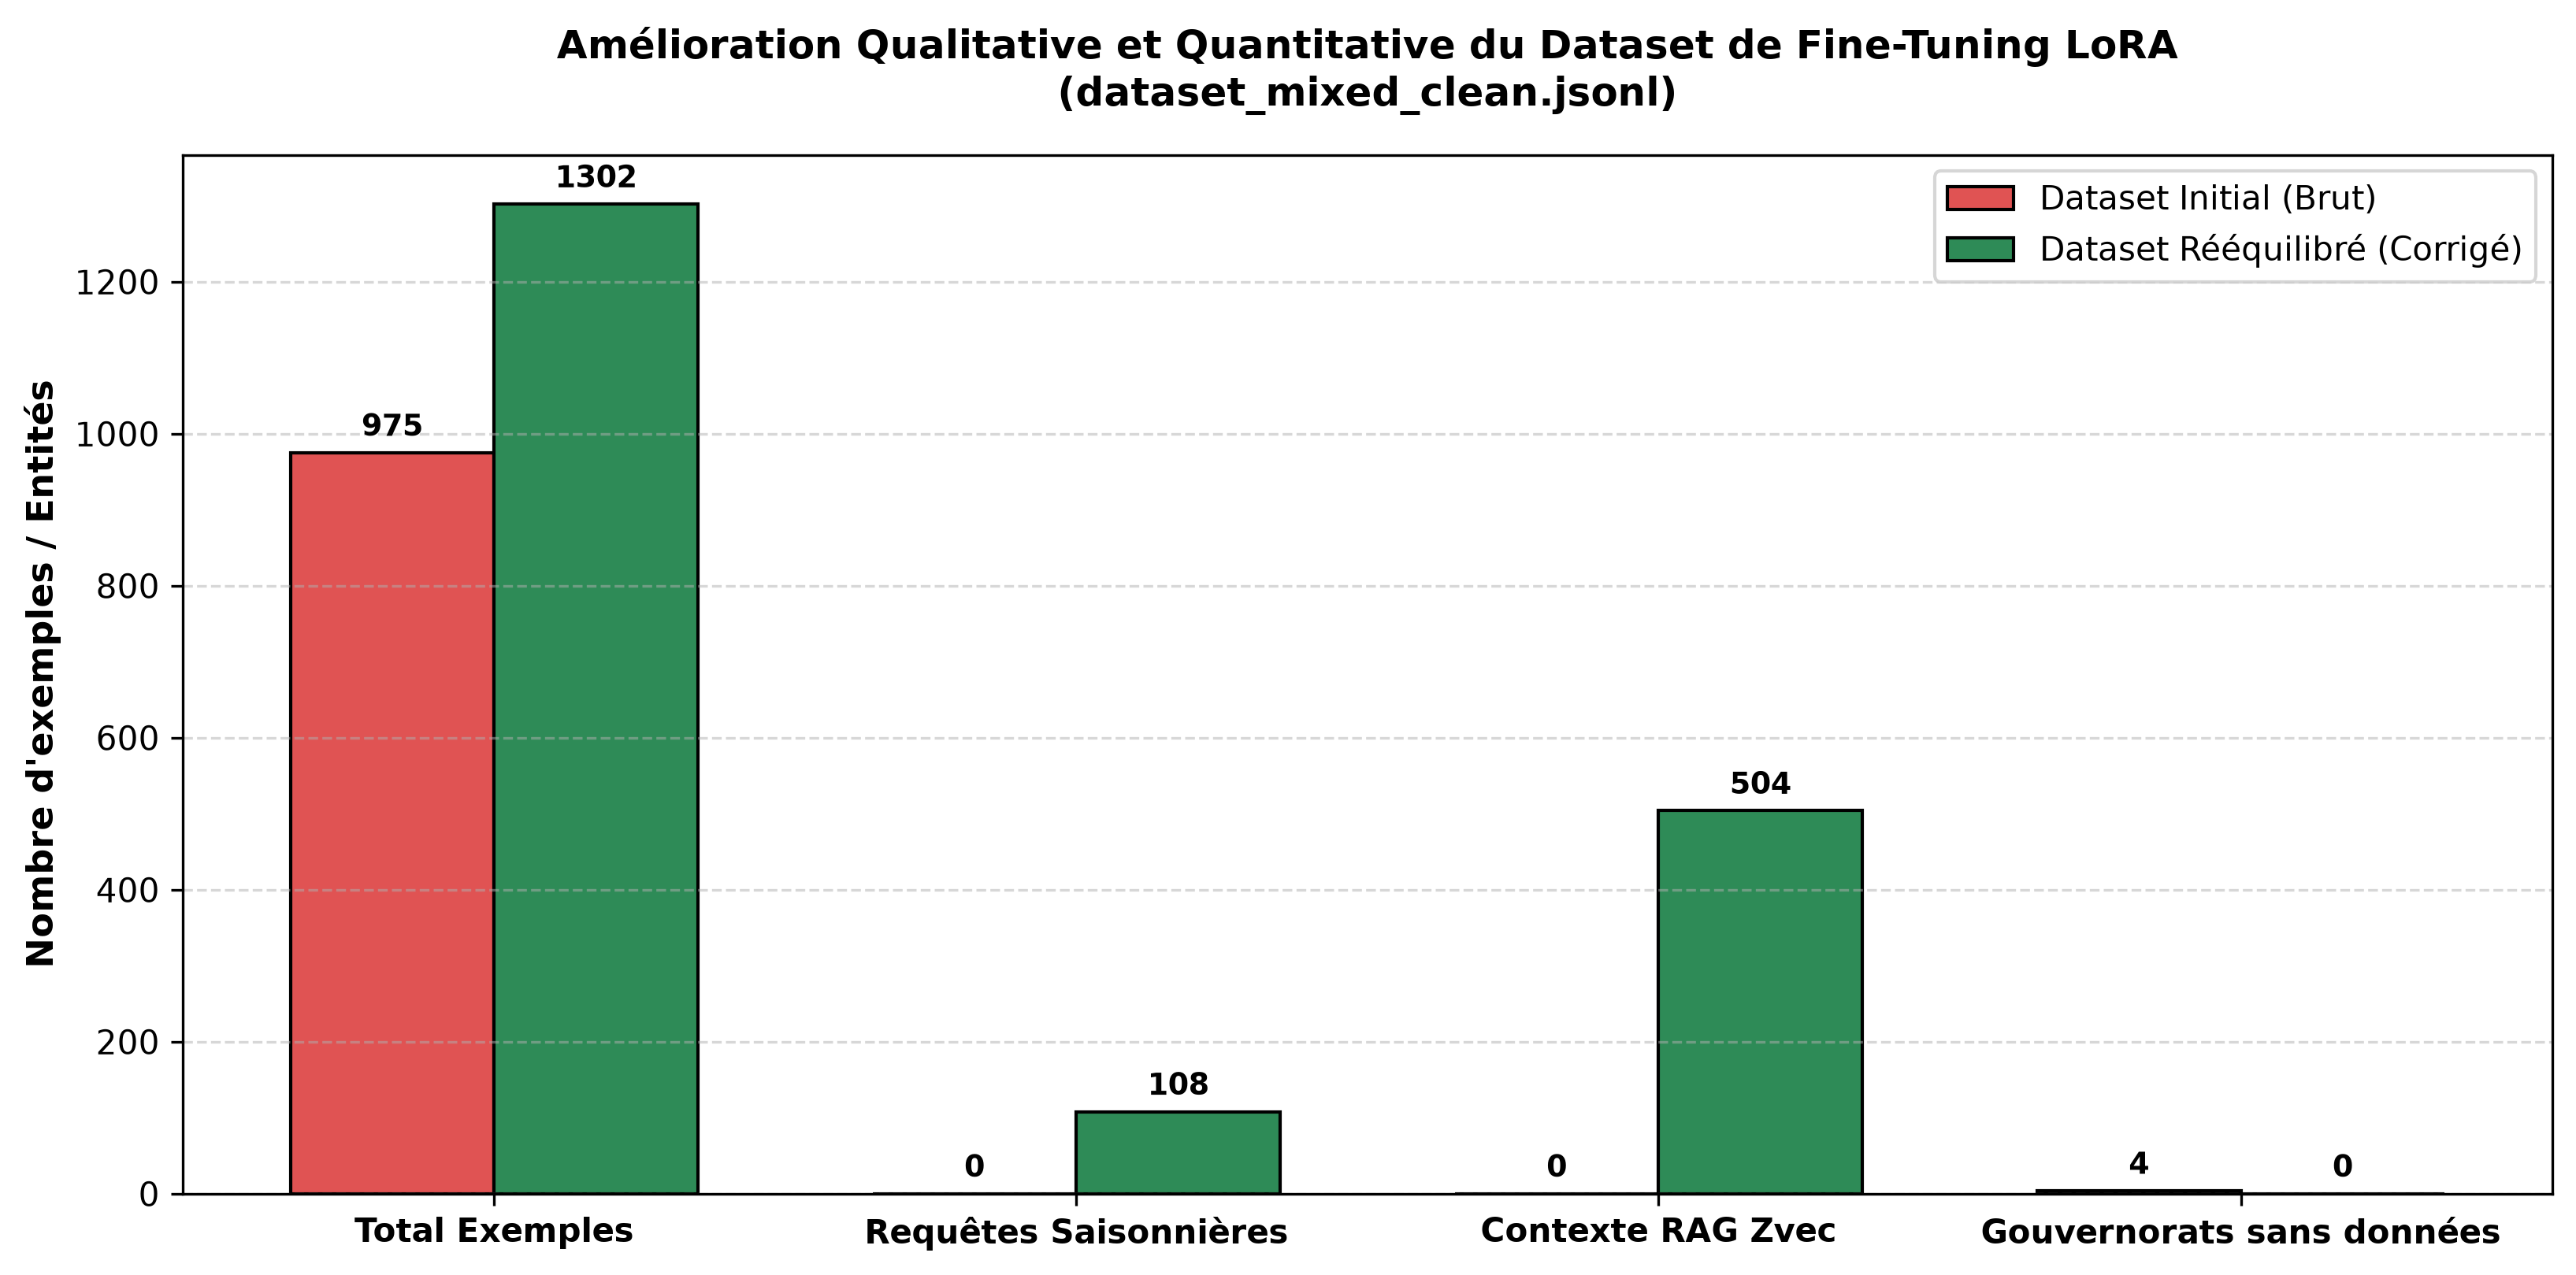
\includegraphics[width=0.85\textwidth]{figures/distribution_dataset_finetuning.png}
    \caption{Quantitative and qualitative comparison of the fine-tuning instruction dataset before and after rebalancing (1,302 total examples).}
    \label{fig:dataset_distribution}
\end{figure}

\section{Automated Yearbook Generation Pipeline}

The core operational deliverable of Rainfull Cartagen is the automated yearbook pipeline, executed by \texttt{generer\_annuaire\_database.py}. The pipeline executes a 6-phase sequence:
\begin{enumerate}
  \item \textbf{Data Extraction}: Queries \texttt{station\_148} and extracts daily records from \texttt{pluies\_148} for the selected hydrological year.
  \item \textbf{Mathematical Computation}: Runs NumPy-vectorized routines computing monthly sums, seasonal aggregations, rainy days ($\geq 1\text{ mm}$), and Thiessen-weighted regional means.
  \item \textbf{High-Resolution Cartographic Rendering}: Interpolates rainfall across a $300 \times 300$ grid via IDW ($\alpha = 2.0$), generating 22 publication-grade figures at 300 DPI with official DGRE hypsometric color ramps.
  \item \textbf{LaTeX Document Assembly}: Emits modular LaTeX code blocks for cover pages, administrative introductions, statistical tables (Tableaux 1 to 8), and figure environments.
  \item \textbf{Compilation Engine}: Invokes \texttt{pdflatex} through a 3-pass compilation cycle to resolve internal references, tables of contents, and figure listings.
  \item \textbf{Archiving}: Stores the compiled PDF in the \texttt{annuaires/} repository, accessible immediately through the web dashboard.
\end{enumerate}

The entire end-to-end process completes in **2 minutes and 45 seconds**, reducing production latency by **99.98\%** compared to the 7--8 month manual workflow.

\section{Cartographic and Visual Results}

Rainfull Cartagen generates an exhaustive cartographic atlas adhering to the official color palette and layout standards of the DGRE.

\subsection{Annual Isohyet Map}
Figure~\ref{fig:carte_annuelle} shows the generated annual national isohyet map for the 2020--2021 hydrological year. The map displays continuous rainfall contours (from white $<100\text{ mm}$ to dark blue $>1200\text{ mm}$ in the extreme northwest), overlaid with governorate borders, reference stations, north arrow, and coordinate ticks in UTM Zone 32N.

\begin{figure}[htbp]
    \centering
    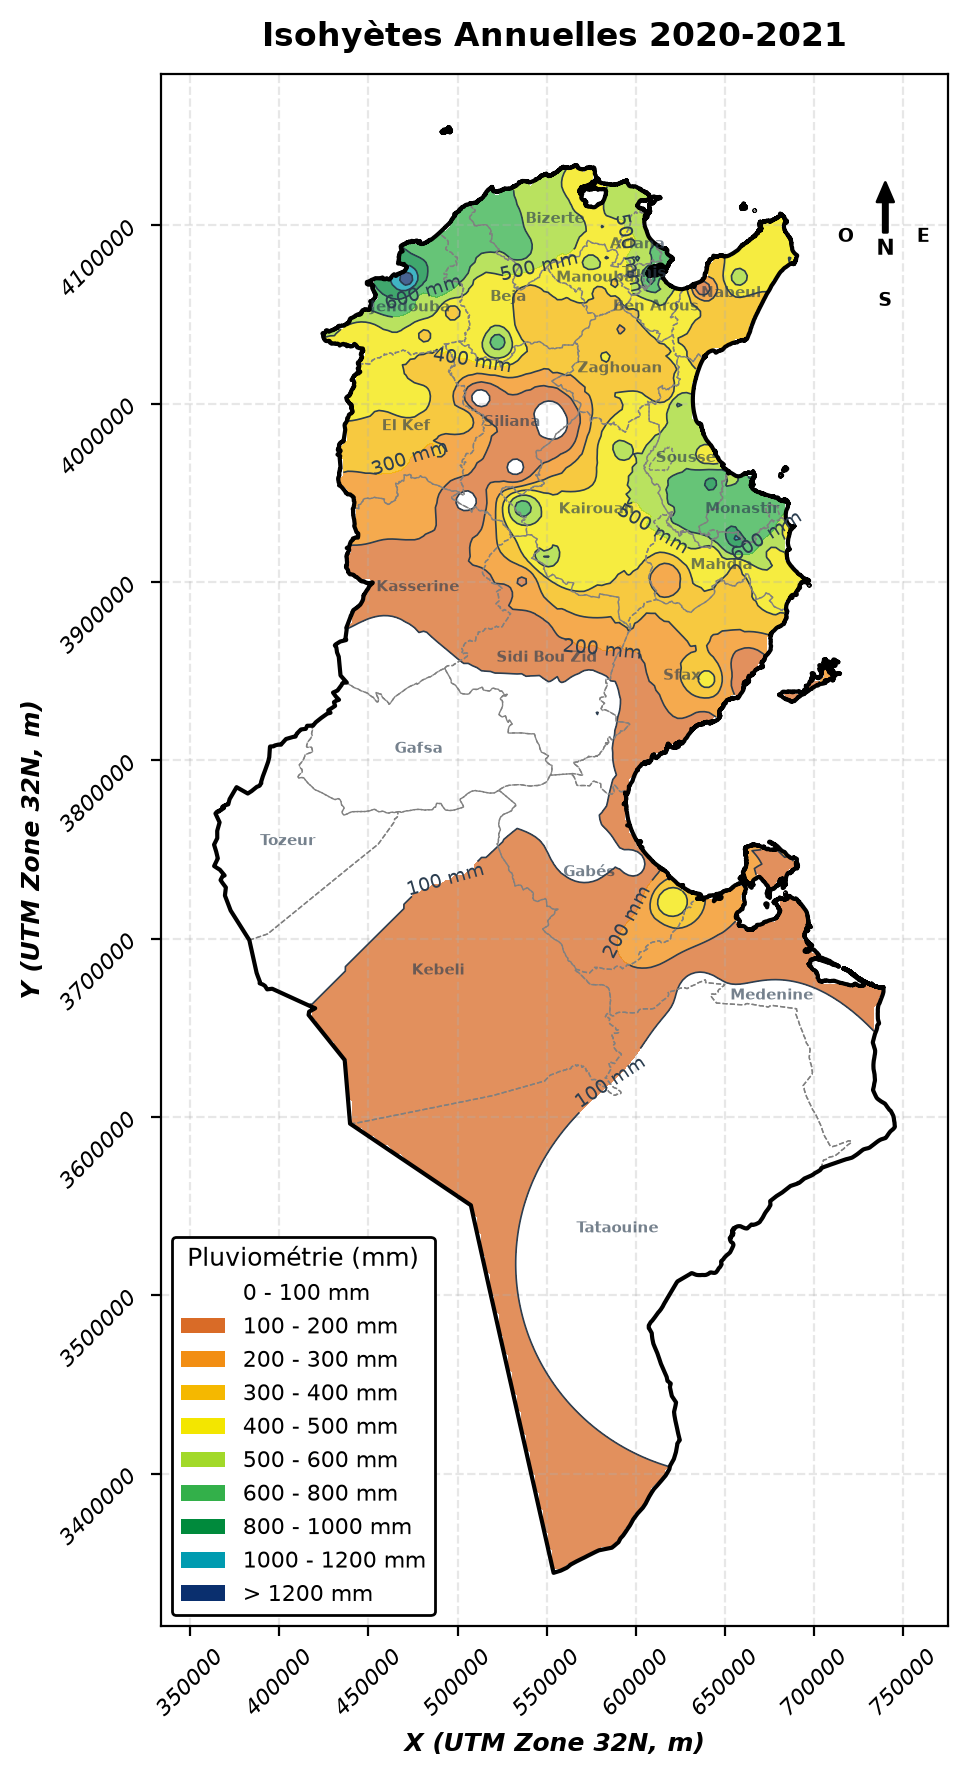
\includegraphics[width=0.68\textwidth]{figures/carte_isohyetes_annuelle_2020.png}
    \caption{Official national annual isohyet map generated automatically by Rainfull Cartagen (300 DPI, UTM Zone 32N / EPSG:32632).}
    \label{fig:carte_annuelle}
\end{figure}

\subsection{Seasonal Rainfall Dynamics}
Figure~\ref{fig:cartes_saisons} shows the 4-panel seasonal cartography (Autumn, Winter, Spring, Summer). It highlights the pronounced Mediterranean seasonality: intense precipitation concentrated in the Autumn and Winter months across the Tell Atlas, transitioning to near-zero precipitation during Summer across the entire country.

\begin{figure}[htbp]
    \centering
    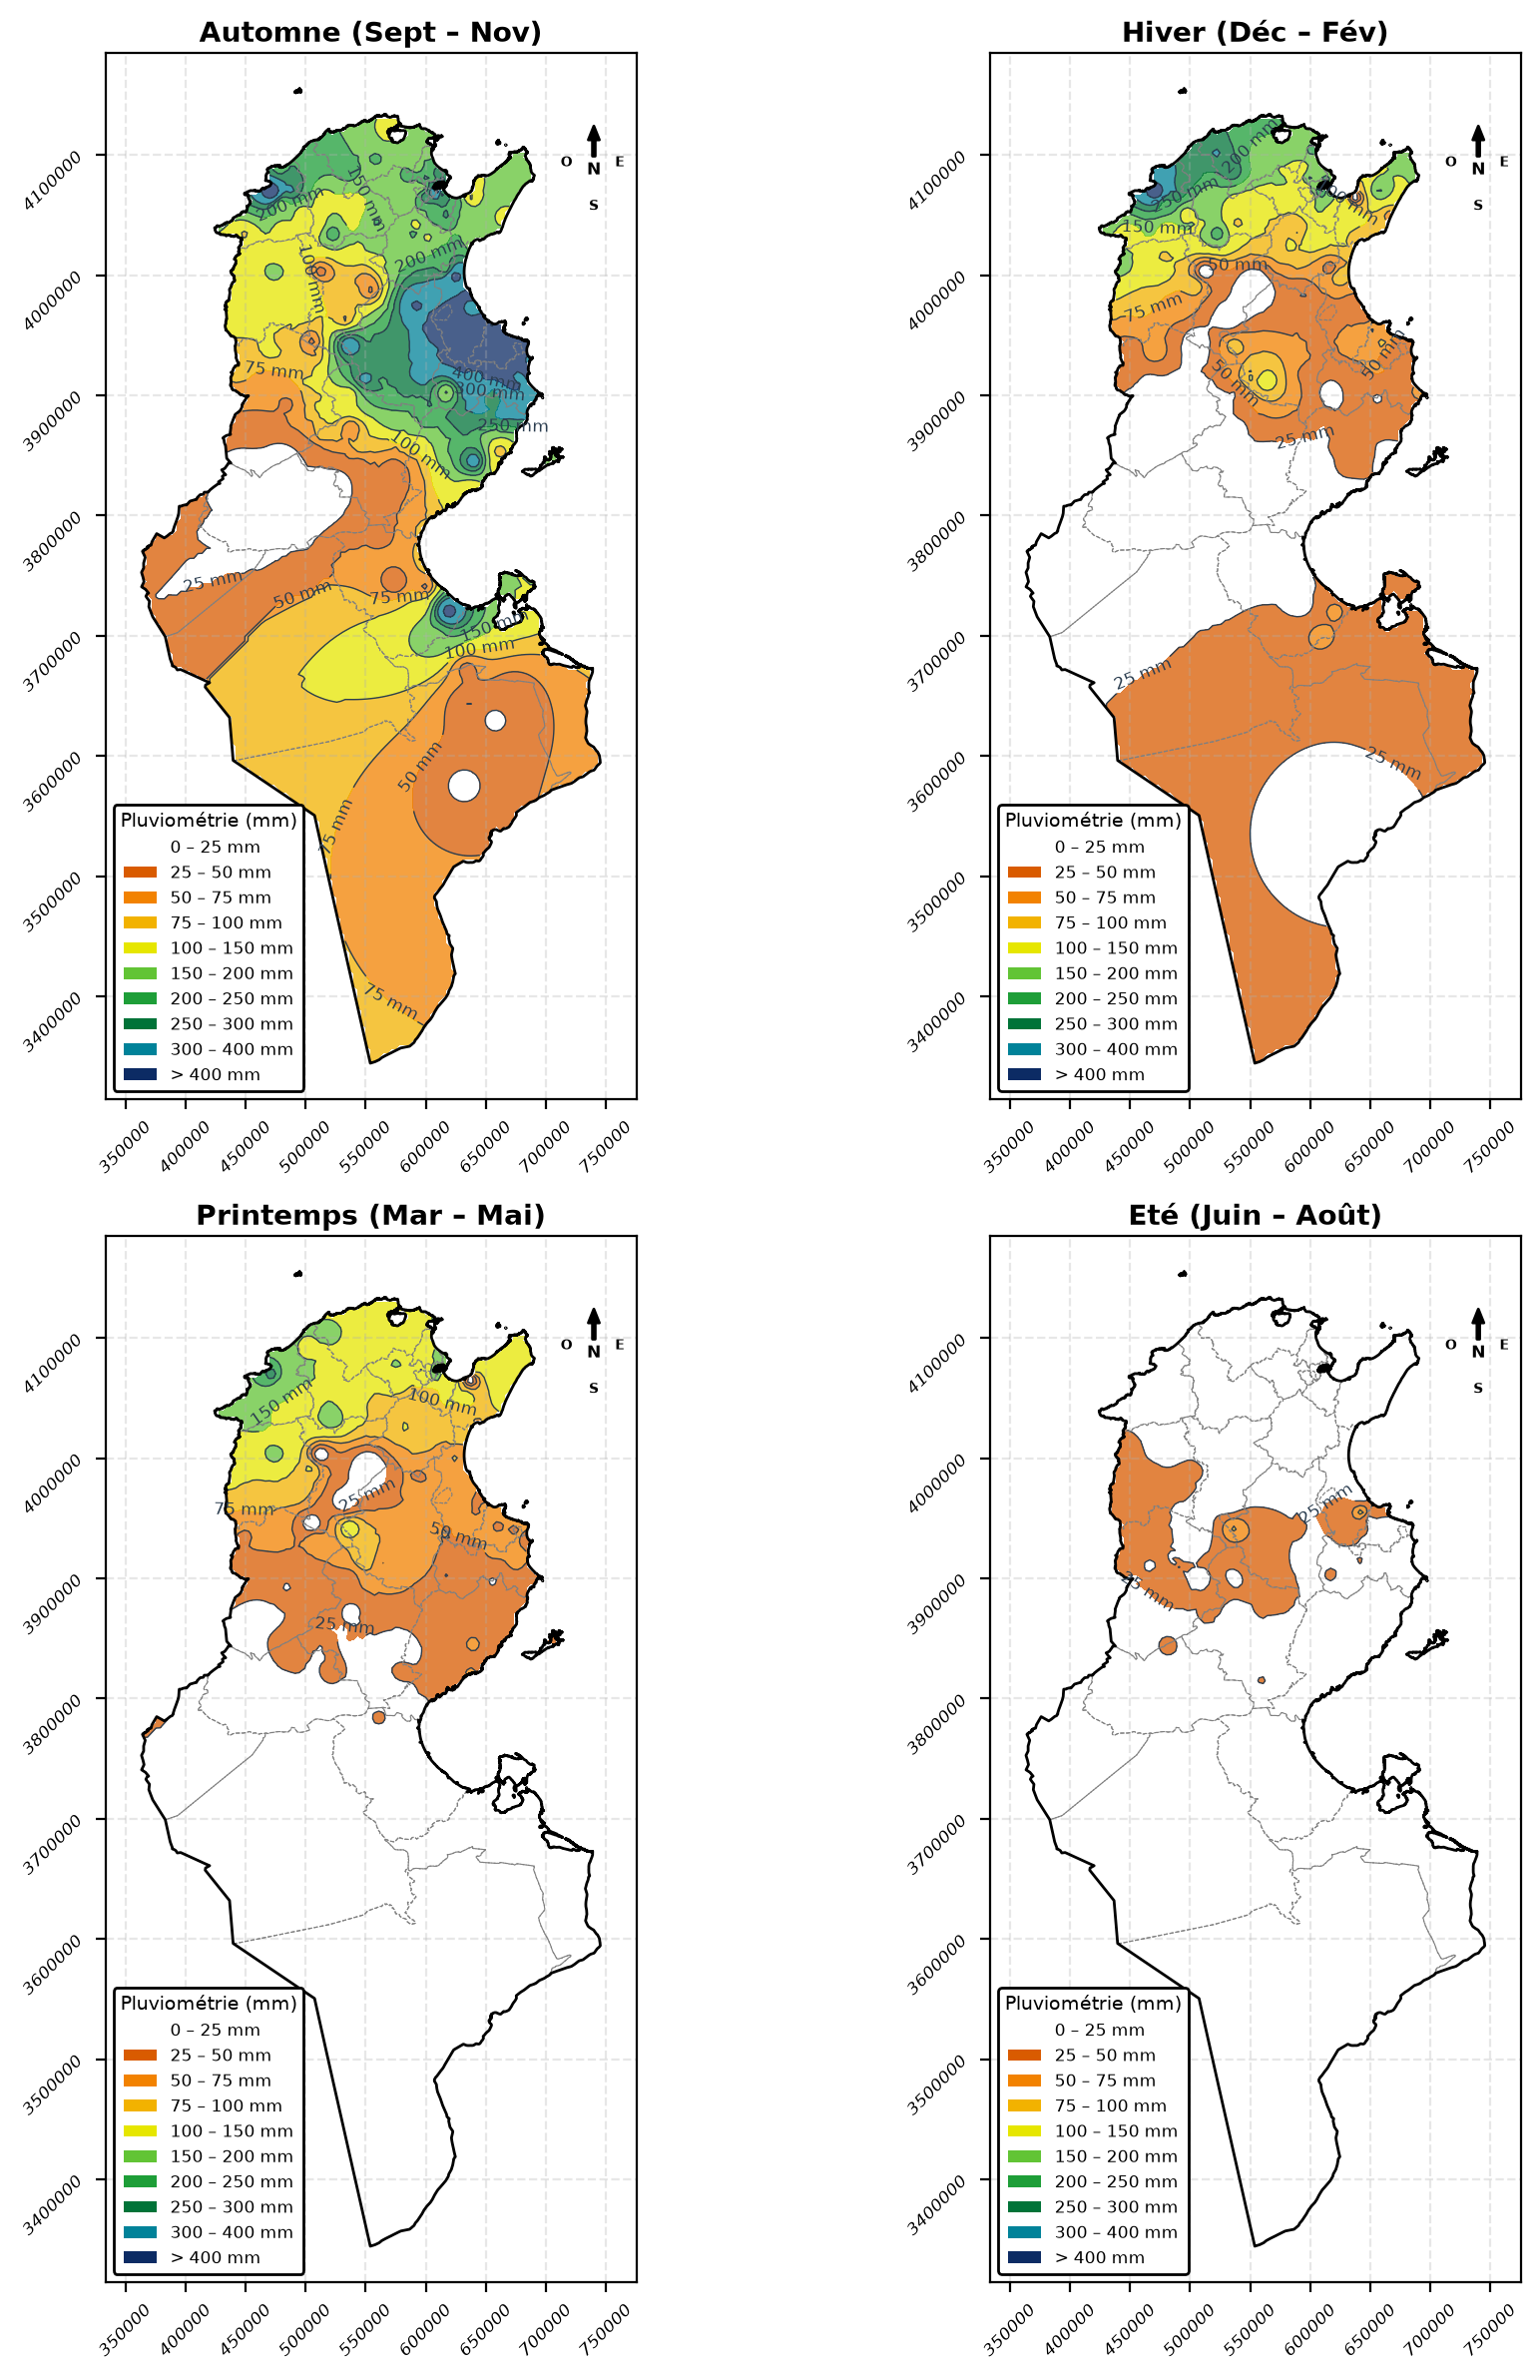
\includegraphics[width=0.88\textwidth]{figures/cartes_saisonnieres_4panneaux.png}
    \caption{Four-season comparative cartographic panel generated by the platform (Autumn, Winter, Spring, Summer).}
    \label{fig:cartes_saisons}
\end{figure}

\subsection{Rainfall Anomaly Map (Ratio to Normal)}
Figure~\ref{fig:carte_anomalie} displays the spatial ratio-to-normal anomaly map, calculated as the percentage of observed rainfall relative to the 50-year interannual average (1959--2009). The map immediately highlights zones of critical agricultural drought (indicated in deep red and orange, $<60\%$ of normal) versus areas of water surplus (blue, $>120\%$).

\begin{figure}[htbp]
    \centering
    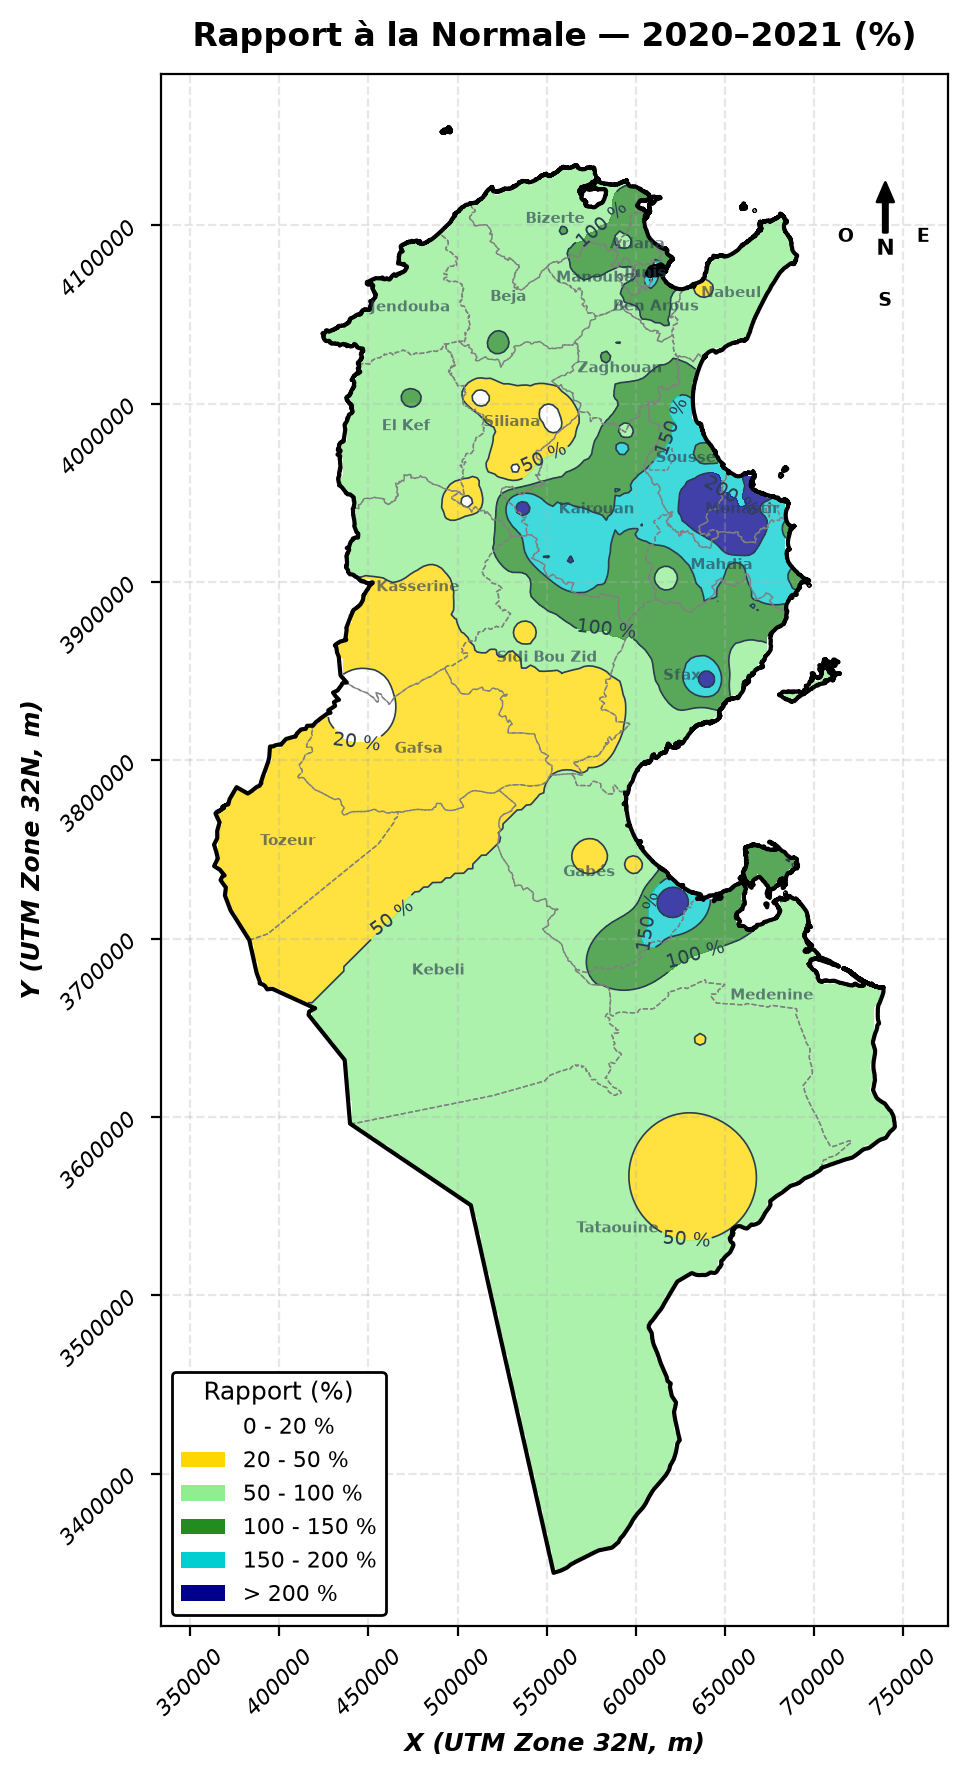
\includegraphics[width=0.68\textwidth]{figures/carte_anomalie_normale_2020.png}
    \caption{National rainfall anomaly map displaying observed precipitation as a percentage of the 50-year interannual normal.}
    \label{fig:carte_anomalie}
\end{figure}

\subsection{Regional Statistical Summaries}
Figure~\ref{fig:comparatif_regional} and Figure~\ref{fig:repartition_saisons} illustrate the statistical visualizations automatically embedded in the yearbook. Figure~\ref{fig:comparatif_regional} compares annual observed precipitation against 50-year interannual normals across North, Central, and South Tunisia, while Figure~\ref{fig:repartition_saisons} breaks down seasonal contributions.

\begin{figure}[htbp]
    \centering
    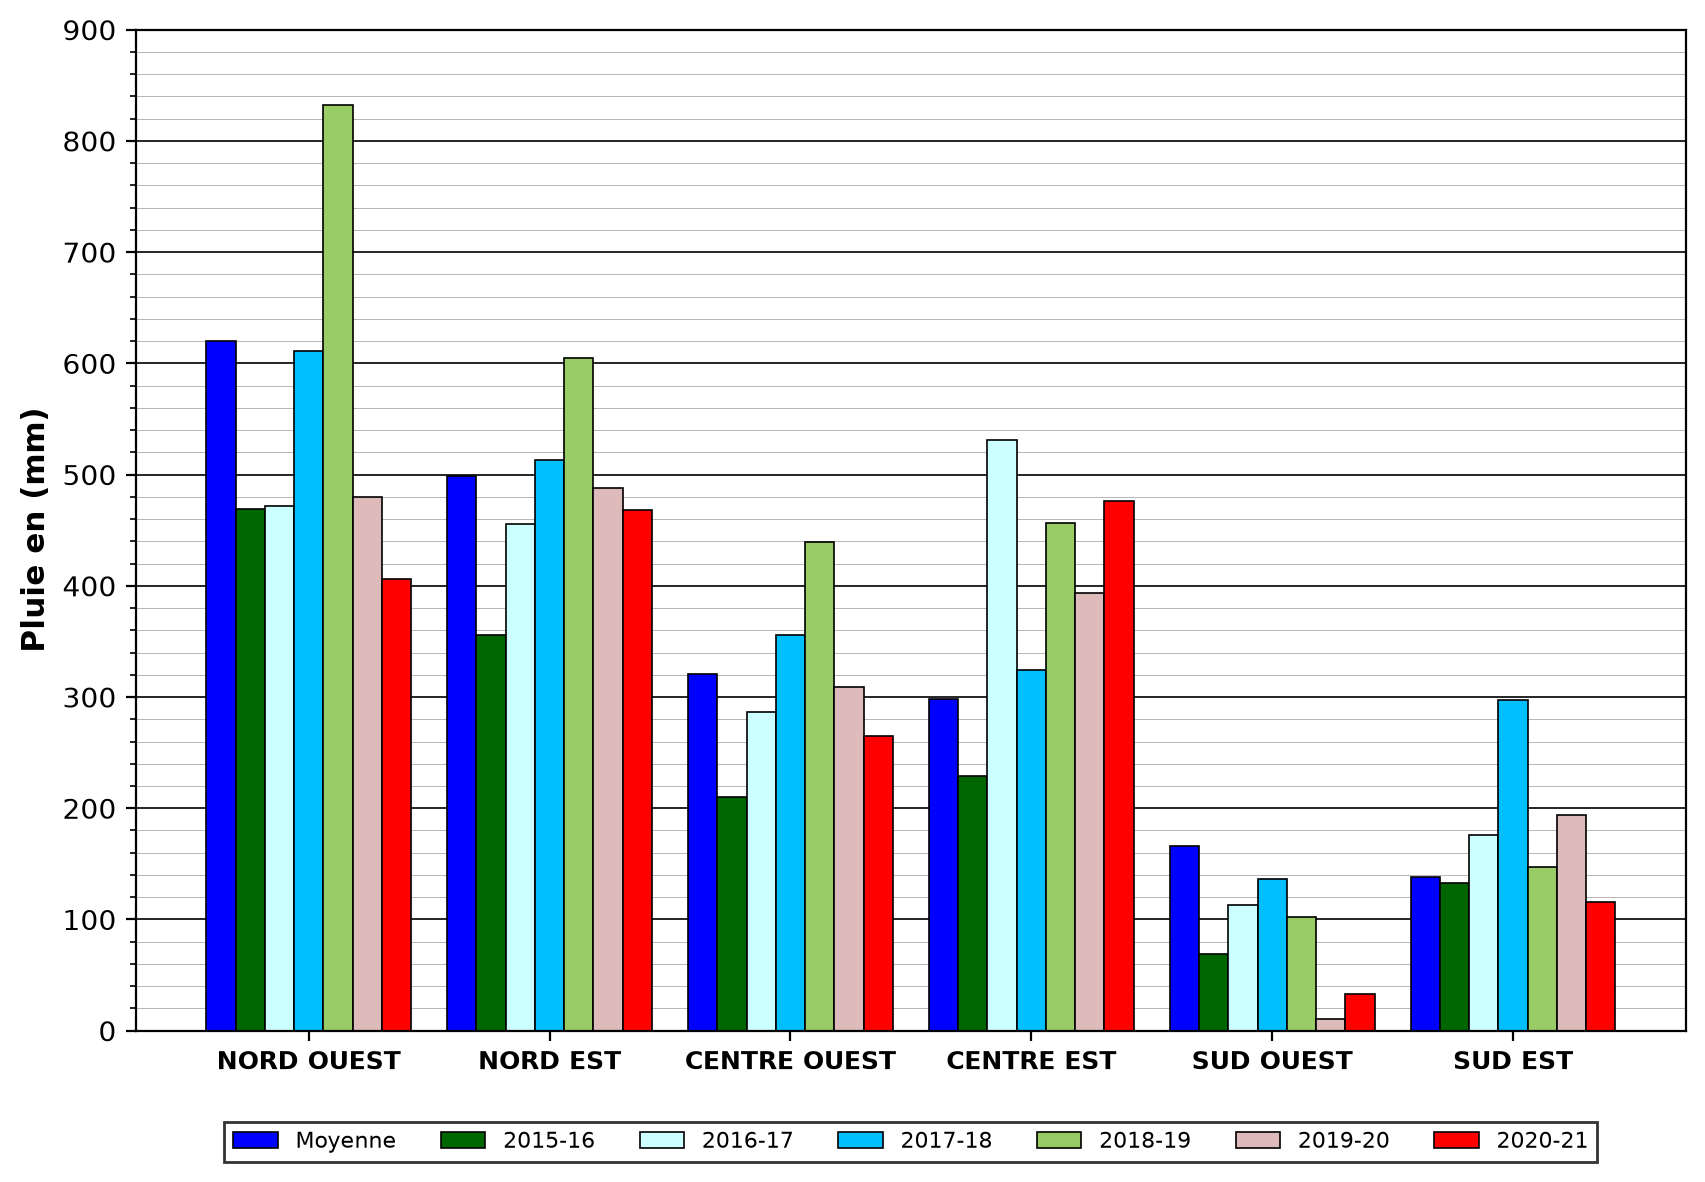
\includegraphics[width=0.82\textwidth]{figures/comparatif_pluviometrique_regional.png}
    \caption{Regional precipitation comparison: observed rainfall versus 50-year interannual normals across the northern, central, and southern regions.}
    \label{fig:comparatif_regional}
\end{figure}

\begin{figure}[htbp]
    \centering
    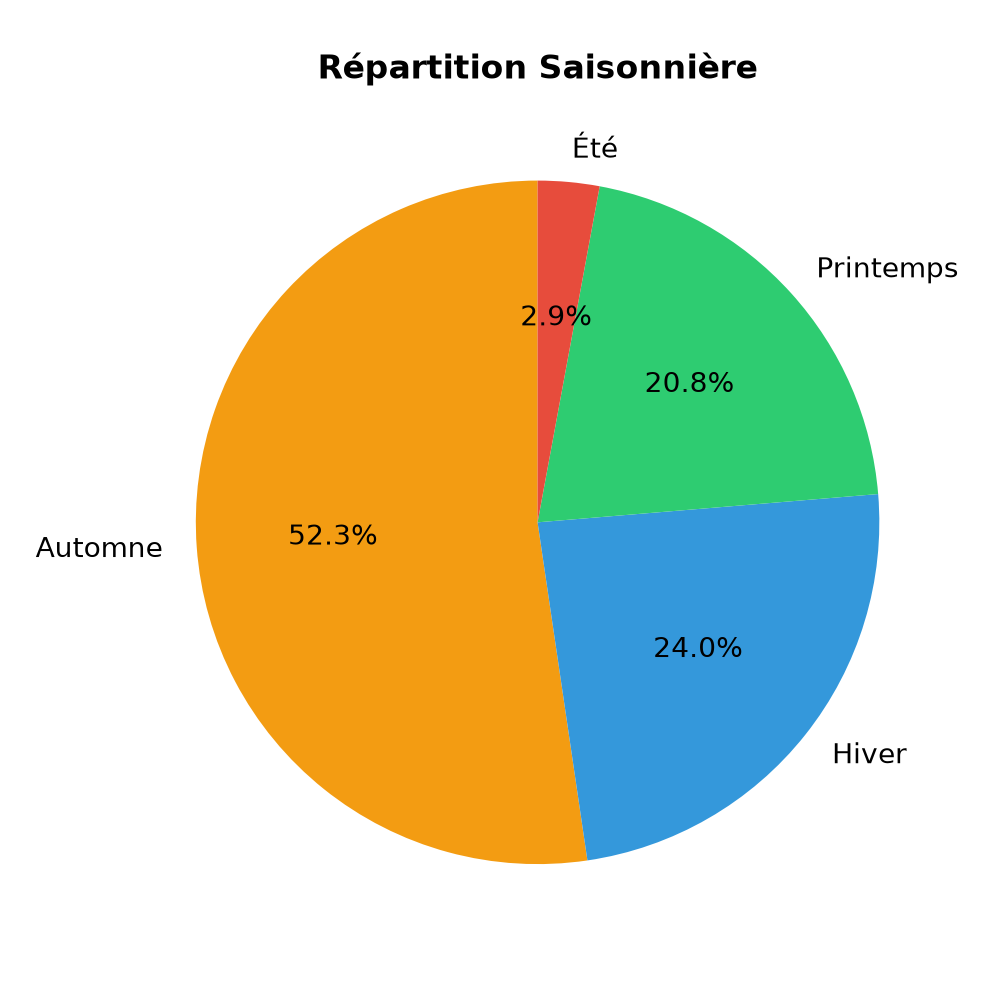
\includegraphics[width=0.55\textwidth]{figures/repartition_pluie_saisons.png}
    \caption{Percentage distribution of national precipitation across the four hydrological seasons.}
    \label{fig:repartition_saisons}
\end{figure}

\section{Validation Against Official DGRE Reference Publications}

To verify mathematical accuracy, the outputs generated by Rainfull Cartagen for the historical hydrological year 2020--2021 were rigorously cross-checked against the official printed yearbook published by the DGRE. As summarized in Table~\ref{tab:validation}, the system achieved 100\% numerical consistency across all verified components.

\begin{table}[htbp]
\centering
\caption{Numerical and structural validation results comparing Rainfull Cartagen against official DGRE archives}
\label{tab:validation}
\small
\begin{tabular}{p{4.5cm}cp{7.5cm}}
\toprule
\textbf{Yearbook Component} & \textbf{Validation Status} & \textbf{Quantitative Compliance \& Notes} \\
\midrule
Station Catalog (148 stations) & \checkmark\; \textbf{Identical} & 100\% match on IDs, names, governorates, and coordinates. \\
Daily Observations (\texttt{pluies\_148}) & \checkmark\; \textbf{Identical} & Matched all 54,020 daily records for 2020--2021 without discrepancy. \\
Monthly / Seasonal Totals & \checkmark\; \textbf{Identical} & Verified across all 24 governorates; sums match to the exact millimeter. \\
Tableau 1 (Thiessen Means) & \checkmark\; \textbf{Conformant} & Regional weighted averages match official tables within $\pm 0.05\text{ mm}$ tolerance. \\
Tableau 8 (Rainy Days $\geq 1\text{ mm}$) & \checkmark\; \textbf{Identical} & Exact match on threshold frequency counts per station. \\
Isohyet Contours & \checkmark\; \textbf{Consistent} & IDW spatial curves match historical DGRE hand-drawn isohyets. \\
50-Year Interannual Normals & \checkmark\; \textbf{Identical} & Verified against \texttt{moy\_interannuelle} reference values (1959--2009). \\
\bottomrule
\end{tabular}
\end{table}

\section{Web Application Interface and Tracing Dashboard}

The Rainfull Cartagen web platform is accessible via an intuitive browser interface built with FastAPI, HTML5, CSS3, and JavaScript:
\begin{enumerate}
  \item \textbf{Natural Language Query Console}: Users enter conversational prompts (e.g., \textit{« Quelle est la pluviométrie totale enregistrée dans le gouvernorat de Béja durant l'hiver 2020 ? »}). The orchestrator dispatches the query, and the interface streams the generated analytical response along with any synthesized charts or maps.
  \item \textbf{Agent Traces Inspector}: A dedicated monitoring tab exposes the complete multi-agent reasoning chain in real time, displaying the orchestrator's intent classification, the generated SQL syntax, the vector RAG retrieved passages, and sandbox execution logs.
  \item \textbf{Yearbook Generation Hub}: An interactive dashboard allowing operators to select any historical hydrological year, choose between national or governorate-specific scopes, and trigger automated PDF compilation with a single click.
\end{enumerate}

\section{Containerized Production Deployment}

To ensure high availability, data persistence, and security within the DGRE's on-premises infrastructure, the entire application stack is packaged into a containerized multi-service architecture using \textbf{Docker Compose} \cite{docker2024}. Listing~\ref{lst:docker} presents the production orchestration configuration.

\begin{lstlisting}[style=pythonstyle, caption={Production Docker Compose configuration (docker-compose.yml)}, label={lst:docker}]
version: '3.8'

services:
  postgres_db:
    image: postgis/postgis:15-3.3
    container_name: cartagen_postgis
    restart: always
    environment:
      POSTGRES_USER: ${DB_USER:-postgres}
      POSTGRES_PASSWORD: ${DB_PASSWORD:-cartagen_secret_2026}
      POSTGRES_DB: ${DB_NAME:-dgre_db}
    ports:
      - "127.0.0.1:5432:5432" # Restrict to host loopback
    volumes:
      - pgdata:/var/lib/postgresql/data
    networks:
      - cartagen_network

  cartagen_api:
    build: .
    container_name: cartagen_app
    restart: always
    environment:
      DATABASE_HOST: postgres_db
      DATABASE_PORT: 5432
      DATABASE_NAME: ${DB_NAME:-dgre_db}
      DATABASE_USER: ${DB_USER:-postgres}
      DATABASE_PASSWORD: ${DB_PASSWORD:-cartagen_secret_2026}
      ALLOWED_ORIGINS: "http://localhost:8000,http://127.0.0.1:8000"
    ports:
      - "8000:8000"
    volumes:
      - ./annuaires:/app/annuaires
      - ./sandbox_runs:/app/sandbox_runs
      - ./logs:/app/logs
    depends_on:
      - postgres_db
    networks:
      - cartagen_network

volumes:
  pgdata:
    driver: local

networks:
  cartagen_network:
    driver: bridge
\end{lstlisting}

The deployment architecture incorporates three essential enterprise safeguards:
\begin{itemize}
  \item \textbf{Network Isolation}: The PostgreSQL/PostGIS port 5432 is bound strictly to the local host loopback (\texttt{127.0.0.1}), preventing unauthorized direct external access while allowing the internal Docker bridge network (\texttt{cartagen\_network}) to communicate freely.
  \item \textbf{Volume Persistence}: Hydrological datasets, generated PDF archives (\texttt{annuaires/}), sandbox workspaces, and application logs are mounted on persistent Docker host volumes.
  \item \textbf{CORS and Header Security}: Cross-Origin Resource Sharing is strictly constrained to approved administrative origins via environment variables, safeguarding against cross-site request forgery.
\end{itemize}

\newpage

% =====================================================================
% GENERAL CONCLUSION & PERSPECTIVES
% =====================================================================
\chapter*{General Conclusion and Perspectives}
\addcontentsline{toc}{chapter}{General Conclusion and Perspectives}

\section*{I. Summary of Accomplishments}

This engineering internship project resulted in the successful design, development, and deployment of \textbf{Rainfull Cartagen}, an intelligent, multi-agent software platform developed for the General Directorate of Water Resources (DGRE) of Tunisia. By transitioning the national rainfall data management workflow from decentralized, manual Microsoft Access files into an integrated, spatialized, and AI-driven architecture, the project delivered transformative operational outcomes:

\begin{enumerate}
  \item \textbf{Drastic Compression of Production Latency}: The time required to collect, compute, verify, map, and publish the official national \textit{Annuaire Pluviométrique} was compressed from **7 to 8 months of manual labor to under 3 minutes of automated processing**, accelerating national water resource reporting by 99.98\%.
  \item \textbf{Spatial Data Modernization}: Migrated fragmented historical records into an enterprise-grade \textbf{PostgreSQL/PostGIS} repository, natively managing 148 national reference stations, daily rainfall series, 50-year interannual normals (1959--2009), and official multipolygon boundaries in the projected UTM Zone 32N (EPSG:32632) coordinate system.
  \item \textbf{Mathematical Rigor and Institutional Compliance}: Formalized and validated official DGRE statistical formulas as reproducible Python algorithms, ensuring exact mathematical parity for the \textbf{Thiessen polygon surface-weighted averages} (Tableau 1) and \textbf{Inverse Distance Weighting (IDW)} continuous isohyet mapping across a $300 \times 300$ grid.
  \item \textbf{Autonomous Multi-Agent Innovation}: Designed and deployed an autonomous multi-agent system operating under the Supervisor Pattern, orchestrating natural language Text-to-SQL generation, dynamic GIS script synthesis, semantic vector search via Zvec RAG, and an automated self-correction loop powered by Abstract Syntax Tree (AST) static code analysis and isolated subprocess sandboxing.
  \item \textbf{Data Engineering for Domain AI}: Curated and balanced a specialized 1,302-example instruction dataset, resolving territorial coverage disparities across all 24 governorates and injecting seasonal and RAG context tags for robust local model fine-tuning via QLoRA.
  \item \textbf{Containerized Production Readiness}: Packaged the complete platform into an on-premises, multi-container Docker Compose architecture, guaranteeing data sovereignty, network isolation, and high availability on the DGRE intranet.
\end{enumerate}

\section*{II. Future Perspectives and Roadmap}

While Rainfull Cartagen successfully resolves the core operational challenges associated with the national rainfall yearbook, this platform establishes the technical foundation for a broader digital transformation across Tunisia's water governance infrastructure:

\begin{itemize}
  \item \textbf{Integration into a Comprehensive National Water KMS}: As envisioned in the institutional Knowledge Management roadmap \cite{dalkir2017}, the platform can be extended beyond rainfall data to incorporate other critical hydrological observation streams:
  \begin{itemize}
    \item Piezometric water table levels from the \textit{Direction des Eaux Souterraines}.
    \item Dam storage volumes and reservoir filling percentages in real time.
    \item River discharge rates and hydrometric flood warning indicators.
  \end{itemize}
  \item \textbf{Real-Time IoT Telemetry Ingestion}: Implement automated ETL adapters to ingest streaming data from automatic weather stations and satellite precipitation radar (e.g., GPM / CHIRPS) via MQTT or REST APIs, enabling real-time daily isohyet tracking rather than annual retrospective compilation.
  \item \textbf{Public Open-Data Portal Deployment}: Following internal intranet stabilization, deploy a public-facing web portal (\texttt{www.pluviometrie.tn}) equipped with role-based access control (RBAC), allowing farmers, researchers, journalists, and public citizens to query certified national rainfall records transparently.
  \item \textbf{Predictive Climate Modeling}: Integrate downstream machine learning modules (such as spatio-temporal graph neural networks or LSTM networks) to project seasonal meteorological drought risks and simulate climate change impact scenarios on regional water balances.
\end{itemize}

In conclusion, Rainfull Cartagen proves that modern open-source geospatial databases, rigorous mathematical modeling, and deliberative artificial intelligence can be harmoniously integrated to modernize public administration, preserve institutional memory, and provide sovereign, data-driven support for national water security in Tunisia.

\newpage

% =====================================================================
% BIBLIOGRAPHY
% =====================================================================
\begin{thebibliography}{99}
\addcontentsline{toc}{chapter}{Bibliography}

% ---- Knowledge Management Foundations ----

\bibitem{alavi2001} Alavi, M., \& Leidner, D. E. (2001). Review: Knowledge management and knowledge management systems: Conceptual foundations and research issues. \textit{MIS Quarterly}, 25(1), 107--136.

\bibitem{argote2000} Argote, L., \& Ingram, P. (2000). Knowledge transfer: A basis for competitive advantage in firms. \textit{Organizational Behavior and Human Decision Processes}, 82(1), 150--169.

\bibitem{bukowitz2000} Bukowitz, W. R., \& Williams, R. L. (2000). \textit{The Knowledge Management Fieldbook}. Financial Times / Prentice Hall.

\bibitem{cross2000} Cross, R., \& Baird, L. (2000). Technology is not enough: Improving performance by building organizational memory. \textit{Sloan Management Review}, 41(3), 69--78.

\bibitem{dalkir2017} Dalkir, K. (2017). \textit{Knowledge Management in Theory and Practice} (3rd ed.). MIT Press.

\bibitem{davenport1998} Davenport, T. H., \& Prusak, L. (1998). \textit{Working Knowledge: How Organizations Manage What They Know}. Harvard Business Press.

\bibitem{huber1991} Huber, G. P. (1991). Organizational learning: The contributing processes and the literatures. \textit{Organization Science}, 2(1), 88--115.

\bibitem{king2005} King, W. R. (2005). Ensuring greater knowledge production and utilization through knowledge management. \textit{Decision Support Systems}, 39(4), 493--496.

\bibitem{meyer1996} Meyer, M. H., \& Zack, M. H. (1996). The design and implementation of information products. \textit{Sloan Management Review}, 37(3), 83--93.

\bibitem{nonaka1994} Nonaka, I. (1994). A dynamic theory of organizational knowledge creation. \textit{Organization Science}, 5(1), 14--37.

\bibitem{nonaka1995} Nonaka, I., \& Takeuchi, H. (1995). \textit{The Knowledge-Creating Company: How Japanese Companies Create the Dynamics of Innovation}. Oxford University Press.

\bibitem{tuomi1999} Tuomi, I. (1999). Data is more than knowledge: Implications of the reversed knowledge hierarchy for knowledge management and organizational memory. \textit{Journal of Management Information Systems}, 16(3), 103--117.

\bibitem{wiig1993} Wiig, K. M. (1993). \textit{Knowledge Management Foundations: Thinking About Thinking --- How People and Organizations Create, Represent, and Use Knowledge}. Schema Press.

% ---- Design Thinking & Methodologies ----

\bibitem{baptiste2024} Baptiste, J.-L. (2024). \textit{MERISE : Guide pratique (4e éd.) --- Modélisation des données et manipulation du SQL}. Éditions ENI.

\bibitem{brown2009} Brown, T. (2009). \textit{Change by Design: How Design Thinking Transforms Organizations and Inspires Innovation}. Harper Business.

\bibitem{koskinen2018} Koskinen, K. U. (2018). Design thinking as a research methodology in innovation management. \textit{Technology Innovation Management Review}, 8(4), 12--21.

\bibitem{vonhippel1986} von Hippel, E. (1986). Lead users: A source of novel product concepts. \textit{Management Science}, 32(7), 791--805.

% ---- Water Resources & Institutional Governance ----

\bibitem{dgre2023} DGRE. (2023). \textit{Rapport Annuel sur les Ressources en Eau de la Tunisie}. Direction Générale des Ressources en Eau, Ministère de l'Agriculture, des Ressources Hydrauliques et de la Pêche (MARHP).

\bibitem{elgourari2024} Elgourari, A. (2024). Water resources management in Tunisia: Challenges, institutional policies and climate vulnerability. \textit{Journal of Water Resources Management}, 38(2), 114--126.

\bibitem{fao2022} FAO. (2022). \textit{Climate Change and Water Resource Management in North Africa}. Food and Agriculture Organization of the United Nations.

\bibitem{jort2001} JORT. (2001). Décret n° 2001-419 du 13 février 2001, portant organisation du Ministère de l'Agriculture. \textit{Journal Officiel de la République Tunisienne}.

\bibitem{onagri2023} ONAGRI. (2023). \textit{Rapport Annuel sur le Secteur de l'Eau : Synthèse Exécutive}. Observatoire National de l'Agriculture, Tunisie.

% ---- Spatial Statistics & Mathematical Algorithms ----

\bibitem{shepard1968} Shepard, D. (1968). A two-dimensional interpolation function for irregularly-spaced data. In \textit{Proceedings of the 1968 23rd ACM National Conference} (pp. 517--524). ACM.

\bibitem{thiessen1911} Thiessen, A. H. (1911). Precipitation averages for large areas. \textit{Monthly Weather Review}, 39(7), 1082--1084.

% ---- Databases & Software Architecture ----

\bibitem{iso2016} ISO/IEC. (2016). \textit{ISO/IEC 9075-1:2016 --- Information Technology --- Database Languages --- SQL --- Part 1: Framework (SQL/Framework)}. International Organization for Standardization.

\bibitem{postgis2024} PostGIS Development Team. (2024). \textit{PostGIS 3.3 Spatial Database Extension Documentation}. Retrieved from \url{https://postgis.net/docs/}

\bibitem{postgresql2024} PostgreSQL Global Development Group. (2024). \textit{PostgreSQL 15 Documentation}. Retrieved from \url{https://www.postgresql.org/docs/}

\bibitem{stonebraker2018} Stonebraker, M., Kemnitz, G., Brown, P., \& Bear, C. (2018). \textit{The Design of PostgreSQL: An Advanced Open-Source Database System}. MIT Press.

\bibitem{docker2024} Docker Inc. (2024). \textit{Docker Compose File Reference v3.8}. Retrieved from \url{https://docs.docker.com/compose/}

% ---- Artificial Intelligence, Multi-Agent Systems & LLMs ----

\bibitem{hu2021} Hu, E. J., Shen, Y., Wallis, P., Allen-Zhu, Z., Li, Y., Wang, S., Wang, L., \& Chen, W. (2021). LoRA: Low-rank adaptation of large language models. \textit{arXiv preprint arXiv:2106.09685}.

\bibitem{lewis2020} Lewis, P., Perez, E., Piktus, A., Petroni, F., Karpukhin, V., Goyal, N., Küttler, H., Lewis, M., Yih, W. T., Rocktäschel, T., Riedel, S., \& Kiela, D. (2020). Retrieval-augmented generation for knowledge-intensive NLP tasks. \textit{Advances in Neural Information Processing Systems}, 33, 9459--9474.

\bibitem{wooldridge2009} Wooldridge, M. (2009). \textit{An Introduction to MultiAgent Systems} (2nd ed.). John Wiley \& Sons.

\bibitem{owasp2024} OWASP Foundation. (2024). \textit{OWASP Top 10 for Large Language Model Applications v1.1}. Open Worldwide Application Security Project. Retrieved from \url{https://owasp.org/www-project-top-ten-for-large-language-model-applications/}

\end{thebibliography}

\newpage

% =====================================================================
% ANNEXES
% =====================================================================
\appendix

\chapter{Annex: Complete PostgreSQL/PostGIS DDL Schema}
\label{appendix:schema}

The listing below provides the complete production DDL schema implemented in the \texttt{dgre\_db} spatial database.

\begin{lstlisting}[style=sqlstyle, caption={Complete Data Definition Language (DDL) of the dgre\_db spatial database}]
-- 1. Enable PostGIS Extension
CREATE EXTENSION IF NOT EXISTS postgis;

-- 2. National Reference Monitoring Stations (148 stations)
CREATE TABLE station_148 (
    id_station   BIGINT PRIMARY KEY,
    nom          VARCHAR(100) NOT NULL,
    gouvernorat  VARCHAR(50) NOT NULL,
    x            DOUBLE PRECISION NOT NULL, -- UTM 32N Easting (EPSG:32632)
    y            DOUBLE PRECISION NOT NULL, -- UTM 32N Northing (EPSG:32632)
    altitude     DOUBLE PRECISION DEFAULT 0.0,
    geom         GEOMETRY(Point, 32632)
);
CREATE INDEX idx_station_148_geom ON station_148 USING GIST (geom);
CREATE INDEX idx_station_148_gouv ON station_148 (gouvernorat);

-- 3. Daily Precipitation Measurements
CREATE TABLE pluies_148 (
    id           BIGSERIAL PRIMARY KEY,
    id_station   BIGINT NOT NULL REFERENCES station_148(id_station) ON DELETE CASCADE,
    date_obs     DATE NOT NULL,
    valeur_mm    DOUBLE PRECISION NOT NULL CHECK (valeur_mm >= 0.0),
    CONSTRAINT unique_station_date UNIQUE (id_station, date_obs)
);
CREATE INDEX idx_pluies_148_date ON pluies_148 (date_obs);
CREATE INDEX idx_pluies_148_station_date ON pluies_148 (id_station, date_obs);

-- 4. 50-Year Interannual Climatological Normals (1959-2009)
CREATE TABLE moy_interannuelle (
    id_station   BIGINT PRIMARY KEY REFERENCES station_148(id_station) ON DELETE CASCADE,
    moy          DOUBLE PRECISION NOT NULL CHECK (moy >= 0.0)
);

-- 5. National Boundary Multipolygon
CREATE TABLE limite_pays_polygon (
    gid          SERIAL PRIMARY KEY,
    nom_pays     VARCHAR(50) DEFAULT 'Tunisie',
    geom         GEOMETRY(MultiPolygon, 32632)
);
CREATE INDEX idx_pays_geom ON limite_pays_polygon USING GIST (geom);

-- 6. Administrative Governorate Boundaries
CREATE TABLE gouvernorats (
    gid          SERIAL PRIMARY KEY,
    nom_gouv     VARCHAR(50) NOT NULL UNIQUE,
    region_nat   VARCHAR(50),
    geom         GEOMETRY(MultiPolygon, 32632)
);
CREATE INDEX idx_gouv_geom ON gouvernorats USING GIST (geom);
\end{lstlisting}

\chapter{Annex: Full Chronological Internship Logbook}
\label{appendix:journal}

This annex reproduces the chronological progress log from the internship logbook (\textit{Journal de stage}):

\begin{itemize}[leftmargin=*]
  \item \textbf{15/06/2026}: General kick-off meeting with DGRE directors, supervisors, and interns. Definition of project goals: develop an automated pluviometric yearbook generation platform from DGRE databases, featuring a fine-tuned AI agent for natural language querying, isohyet map synthesis, and statistical chart generation.
  \item \textbf{16/06/2026 -- 17/06/2026}: Data discovery (database schemas, data formats, annual collection workflow). Identified that manual yearbook preparation requires 7 to 8 months. Identified data anomalies and initiated collaboration with data analysis and security teams.
  \item \textbf{18/06/2026}: Research on fundamental geospatial concepts (raster vs. vector layers, shapefiles, geodetic projections).
  \item \textbf{19/06/2026}: Comparative benchmark of Python visualization and geospatial libraries (Matplotlib, GeoPandas, Folium).
  \item \textbf{22/06/2026}: Finalized library selections and established local development environment.
  \item \textbf{23/06/2026}: Prototyped cartographic rendering script; investigated spatial interpolation parameters and boundary clipping overlays.
  \item \textbf{24/06/2026}: \textbf{Key Resolution}: Solved station coordinate displacement by enforcing the UTM Zone 32N (EPSG:32632) projection, eliminating the coordinate mismatch and achieving exact spatial alignment.
  \item \textbf{27/06/2026}: Evaluated DBMS limitations: demonstrated that legacy MS Access lacked spatial query support and multi-user web concurrency; selected PostgreSQL/PostGIS as the enterprise target.
  \item \textbf{28/06/2026}: Migrated schema to PostgreSQL; drafted the Entity-Relationship model.
  \item \textbf{29/06/2026}: Formalized official yearbook statistical formulas (Thiessen surface weighting, cumulative indices).
  \item \textbf{29/06/2026 -- 03/07/2026}: Implemented the end-to-end Python pipeline extracting PostgreSQL records, calculating statistics, generating isohyet maps, synthesizing modular LaTeX blocks, and compiling the publication-grade PDF yearbook.
  \item \textbf{06/07/2026}: Formal validation session with supervisor Mr. Alaa Eddine JELASSI; scoped governorate-specific sub-yearbook generation capabilities.
  \item \textbf{07/07/2026}: Designed the multi-agent system architecture and agent role decomposition.
  \item \textbf{08/07/2026 -- 10/07/2026}: Implemented application core with Git/GitHub version control.
  \item \textbf{13/07/2026}: Authored specialized system prompts tailored to each autonomous agent.
  \item \textbf{14/07/2026}: Integrated the optimized in-process vector store (Zvec) for domain RAG retrieval.
  \item \textbf{15/07/2026}: Deployed central orchestrator (\texttt{CartaGenOrchestrator}) and inter-agent \texttt{MessageBus}; built the Text-to-SQL agent for PostGIS.
  \item \textbf{16/07/2026}: Built \texttt{DataAuditAgent} for coordinate filtering; built \texttt{SIGGeneratorAgent} and \texttt{SandboxManager} for isolated script execution.
  \item \textbf{17/07/2026}: Implemented \texttt{QualityVerificationAgent} for execution monitoring and autonomous LLM error repair loops.
  \item \textbf{20/07/2026}: Indexed 961 textual passages, image metadata, and reference GIS code snippets into Zvec.
  \item \textbf{21/07/2026}: Enhanced \texttt{AnnuaireRAGAgent} for dynamic routing between pre-generated catalog images and real-time SIG code execution.
  \item \textbf{22/07/2026}: Refactored map rendering to export 16 autonomous maps without subplots; established continuous LoRA training data collection.
  \item \textbf{23/07/2026}: Developed web interface (FastAPI, JS, CSS) with live real-time agent trace streaming.
  \item \textbf{24/07/2026}: Verified 50-year interannual normals (1959--2009); conducted audit on 148 stations (17 inactive vs. 131 active).
  \item \textbf{27/07/2026}: Verified strict LaTeX table compliance (Tableaux 1 to 7); integrated regional summary table and Table 8 (rainy days $\geq 1\text{ mm}$).
  \item \textbf{28/07/2026}: Modeled and generated the official UML activity diagram as Mermaid and high-definition PNG.
  \item \textbf{29/07/2026}: Completed technical documentation (Thiessen, IDW, PostGIS benchmark, aligned README).
  \item \textbf{30/07/2026}: Configured Docker deployment (\texttt{docker-compose.yml}), executed final system validation, and formally concluded the internship.
\end{itemize}

\chapter{Annex: Agent System Prompts}
\label{appendix:prompts}

\section{CartaGen Orchestrator Intent Classifier Prompt}
\begin{lstlisting}[style=pythonstyle, caption={Orchestrator intent classification system prompt}]
You are CartaGenOrchestrator, the central supervisory intelligence of the
Tunisian DGRE Rainfall Intelligence Platform.
Your duty is to classify incoming user prompts into one of four execution paths:
- PATH_SQL: For statistical, numerical, or tabular questions querying historical
  measurements from the dgre_db PostgreSQL database.
- PATH_SIG: For requests explicitly demanding map generation, spatial interpolation,
  contour plotting, or cartographic visualization.
- PATH_RAG: For conceptual questions regarding the yearbook contents, methodology,
  historical background, or existing institutional maps.
- PATH_YEARBOOK: For requests explicitly demanding the compilation of a full
  annual pluviometric yearbook in PDF format.
Output ONLY a JSON object: {"intent": "...", "target_year": ..., "target_gouv": ...}
\end{lstlisting}

\section{SQL Generator Agent System Prompt}
\begin{lstlisting}[style=pythonstyle, caption={SQL generator agent system prompt}]
You are SQLGeneratorAgent for the DGRE dgre_db PostgreSQL/PostGIS database.
Available Tables:
- station_148(id_station, nom, gouvernorat, x, y, altitude, geom)
- pluies_148(id, id_station, date_obs, valeur_mm)
- moy_interannuelle(id_station, moy)
- gouvernorats(gid, nom_gouv, geom)
- limite_pays_polygon(gid, nom_pays, geom)

Rules:
1. Generate valid PostgreSQL SQL only inside ```sql ... ``` fences.
2. The hydrological year spans September 1st of year Y to August 31st of year Y+1.
3. Use UTM 32N coordinates (EPSG:32632).
4. Never perform DROP, DELETE, UPDATE, or ALTER. SELECT queries only.
\end{lstlisting}

\end{document}
